\lchapter[acquisition]{Data collection framework}

\section{Introduction}

\p{Open-source projects and data availability}
The process of modeling, visualizing, and analyzing any type of system, whether complex or not, presupposes the availability of the data set describing the system and the processes evolving around its development. In this respect, by choosing to focus our work on open-source software projects, we can take advantage of the fact that data about their development process is readily available online. Moreover, the system itself can also be processed automatically to gather different kinds of information (e.g., the identification of dependencies between its components).

\p{Need for data aggregation}
The open-source nature of the analyzed projects almost guarantees the \emph{availability} of the necessary data. This just makes the analysis task \emph{possible}, not necessarily easy. In fact, the different data sets are often scattered over a plethora of different systems, represented by the tools that the development teams chose for the task. For example, a project could make use of a source code repository to coordinate the different versions of the codebase, an issue tracker to gather the outstanding bugs and features to be added to the product, a mailing list for discussions between developers, and a chat service for conversations requiring rapid feedback loops. Before beginning the analysis process, data from the selected sources will have to be aggregated and stored in a conventional format.

\p{Data source types, implementations and plugins}
Data sources can vary by type (e.g., source code repository, mailing lists, issue trackers,\ldots) and then by implementation (e.g., GIT, SVN and CVS are all possible source code repository managers). Given the multitude of options and the endless combinations they could be arranged in, we renounced to implement a system covering every possible solution. On the other hand, limiting ourselves to a fixed configuration is not an acceptable solution either, as this would reduce the number of projects we will be able to analyze. Instead, we chose to provide a generic \emph{data acquisition framework} which can be exploited by custom, data-source specific, plugins. We also developed some plugins for the projects we used as test cases.

\p{Structure of this chapter}
In the remaining part of this chapter, we will first discuss the analysis of the framework to be
developed (\ref{sec:acquisition/analysis}), followed by the presentation of the architectural design required to achieve the
desired extensibility (\ref{sec:acquisition/design}). In the last two sections, we first highlight interesting implementation
details (\ref{sec:acquisition/implementation}), and then terminate with a summary of the results (\ref{sec:acquisition/results})
with particular interest with regard to the different data collector implementations.


\section{Analysis}
\label{sec:acquisition/analysis}

\subsection{Data sources}
\label{sec:acquisition/analysis/sources}

\p{Introduction}
As we already discussed in the introduction to the present chapter, the data needed for the analysis of a system may come from different sources. These sources can vary by \emph{type} and then by \emph{implementation}. Normally, a single data source contains data belonging to one or two domains, and two data sources of the same kind provide data from the same domains even if their implementation differs.

\p{Data sources}
\Vref*{tab:sources} lists some of the possible data sources that can be used to gather data about the development process of a software product. It is important to note that our focus on \emph{open-source} projects derives from these systems to be freely accessible over the Internet, but all considerations expressed in the present document also apply to closed-source products. The only requirement is that the organization uses a system to collect the information needed for the analysis process and that the data can be extracted from it in an automated way.

\begin{table}
  \begin{threeparttable}
  \begin{tabularx}{\textwidth}{ p{2.3cm} | X | X }
    \toprule
    Type & Domain(s) & Possible implementations\tnote{1}\\[.7mm]
    \hline

    Source code & Component dependencies & Any programming language (C, C++, Java, Python, \ldots \\[3mm]
    Version control software & Affection of developers to components, Historical evolution & GIT, SVN, CVS, Mercurial, Bazaar, Perfoce, Darcs, \ldots \\[3mm]
    Email & Communication patterns (long-term decisions) & Email inboxes (\gls{pop3}, \gls{imap}) or mailing list softwares (Mailman, GroupServer, EGroups, \ldots) \\[3mm]
    Chat/\gls{voip} & Communication patterns (rapid feedback) & \gls{irc}, \gls{xmpp}, \gls{voip}, LanTalk, \ldots \\[3mm]
    Issue tracker & Change requests & Bugzilla, Trac, Teamwork, JIRA, Redmine, \ldots \\

    \bottomrule
  \end{tabularx}
  \vspace{1mm}
  \begin{tablenotes}
  \item [1] \footnotesize{We use the term \emph{implementations} to refer to a specific kind of the data source type in exam.}
  \end{tablenotes}
  \end{threeparttable}

  \caption[Possible data source types, domains and implementations]{List of some possible data sources which can be used to gather data about software projects.}
  \label{tab:sources}
\end{table}

\subsection{From raw to aggregated data: collectors and acquisition sessions}

\p{Collectors}
In the introduction we anticipated that the acquisition system is composed by many different plugins, each one targeting a different data-source kind and implementation (examples thereof presented in \vref{sec:acquisition/analysis/sources}). We call such a plugin a \emph{data collector} or simply \emph{collector}. The job of a collector is, given a configuration as input, retrieve the data from the data source, transform it as necessary, and output a multi-domain graph in the format described in \vref{sec:case/tech}.

\p{Acquisition sessions}
The analysis of a given project normally requires data coming from more than one source. The set of collectors (and related configuration) to acquire the data for a given project is called an \emph{acquisition session}. Acquisition sessions can be managed through the web interface and are persistent. An acquisition session holds both the configuration and the eventual result of its execution.

\p{Collectors execution}
For convenience, collectors can either be run in batches as part of an acquisition session, or manually by executing a shell command. Means are also provided to directly invoke the respective functions to allow the integration of collectors in third party libraries.

\p{Execution orchestration}
When executed in batches, collector runs are orchestrated through a specific service, called \emph{acquisition server} (or \emph{collection server}). The task of this component is similar to a job queue: it accepts incoming commands, runs them asynchronously, and finally communicates the results back to the invoking part.

\p{Data merging}
Once the results from each collector in an acquisition session are received, the respective graphs are merged into a single multi-domain graph. The individual results, as well as the merged graph, are all accessible through the acquisition session.

\subsection{Use case diagram}

\p{Introduction}
The previous subsection illustrated the high-level components of the acquisition framework and introduced two ways in which an end user can interact with them, namely the web application and the command line. In this subsection we introduce the use case diagram for the acquisition process, as illustrated in \ref{fig:uc-acquisition}, \ref{fig:uc-server} and \vref{fig:uc-collector}.

\begin{figure}[p]
  \begin{adjustwidth}{-2.2cm}{-1.5cm}
  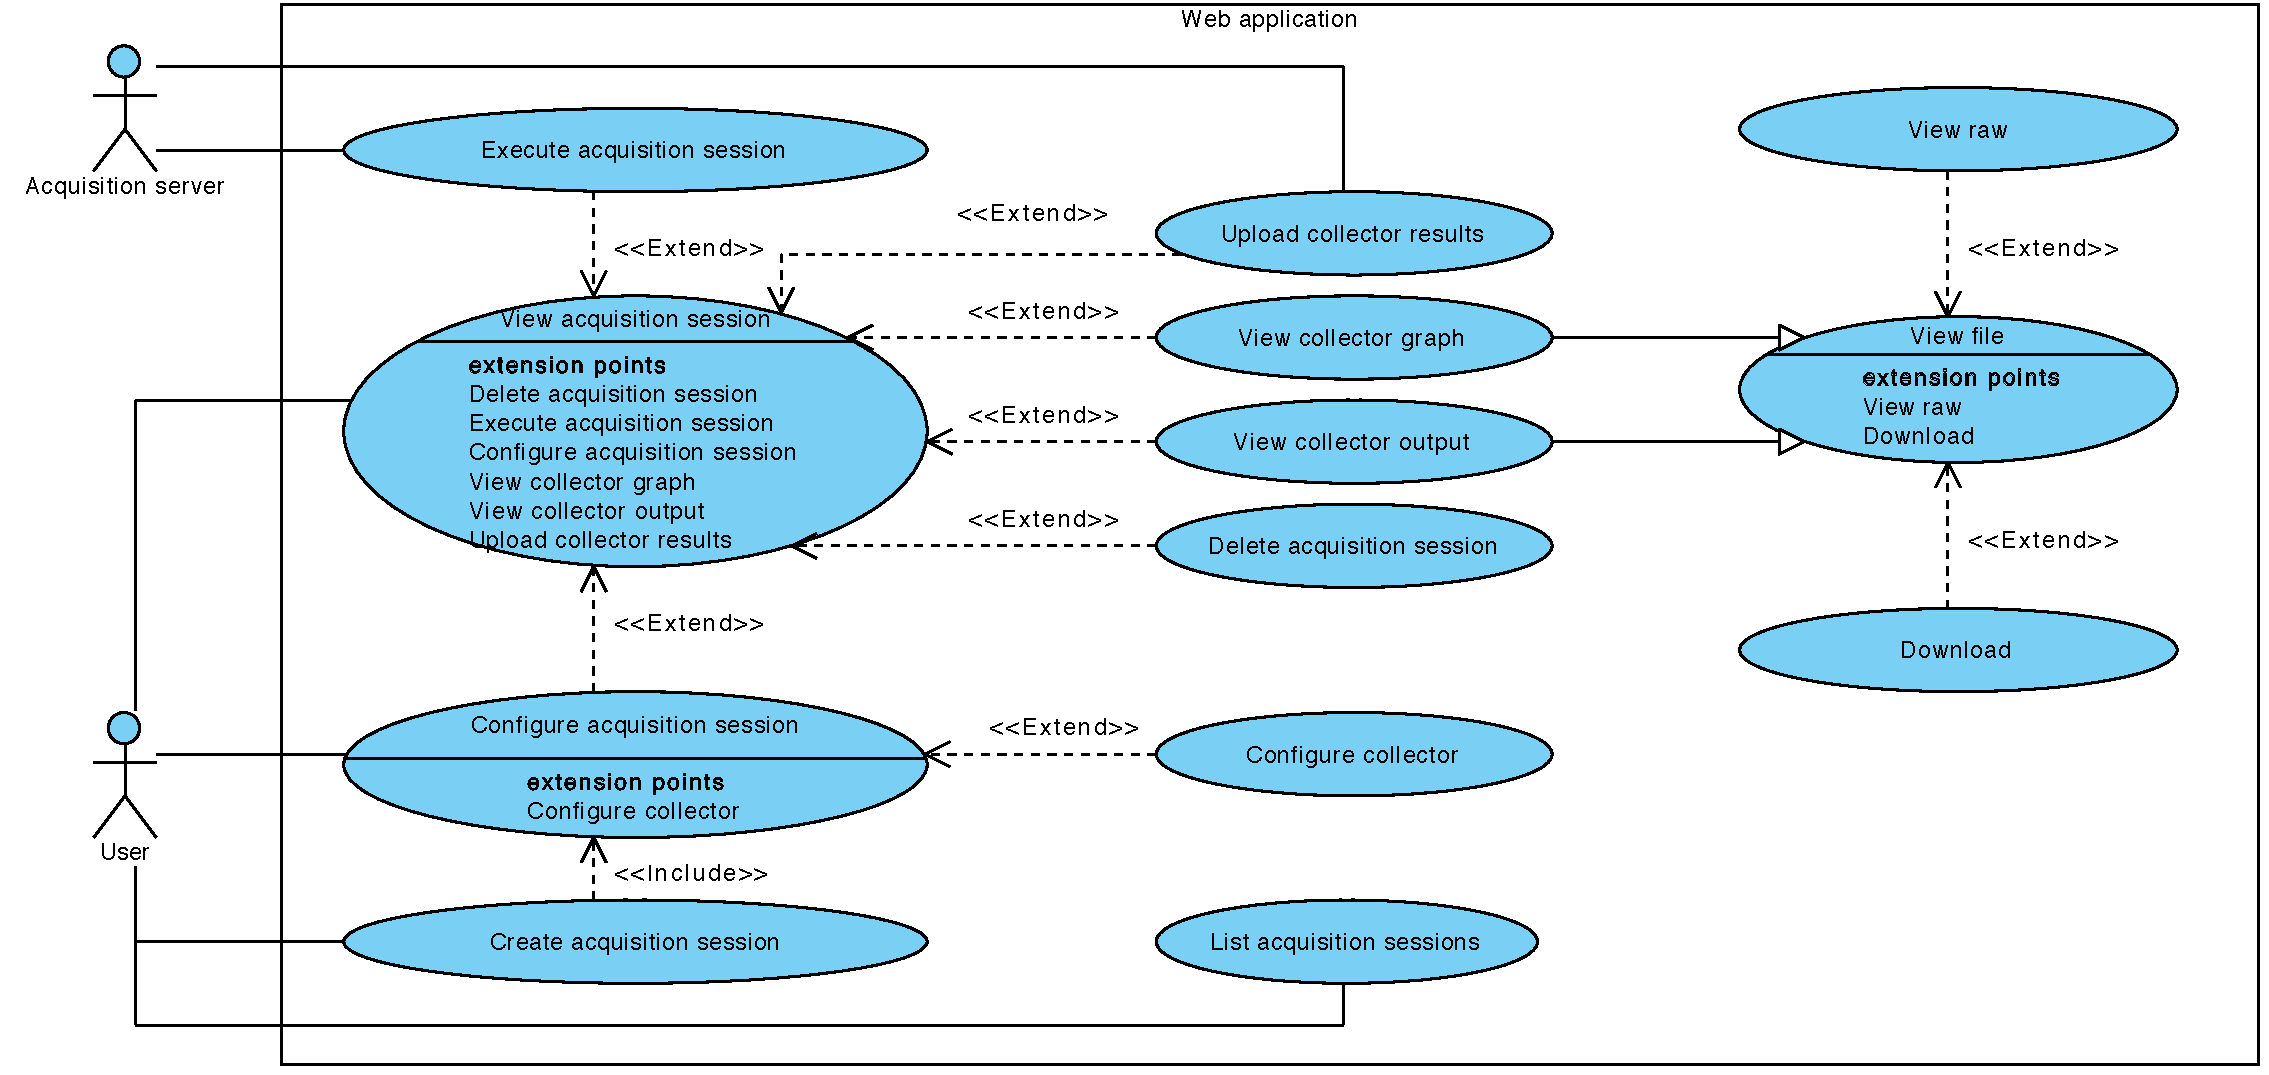
\includegraphics[width=\linewidth]{images/diagrams/uc-acquisition}
  \end{adjustwidth}

  \caption[Use case diagram for the data acquisition web application.]{Use case diagram for the data acquisition web application.}
  \label{fig:uc-acquisition}
\end{figure}

\p{Actors}
For the purposes of the analysis, the acquisition framework can be split in three subsystems. We analyze these three subsystems independently, each time considering the other two subsystems as actors interacting with the current subject. The three subsystems, and thus the actors presented in the use case diagrams, can be described as follows:

\begin{description}
  \item[Web application] This is the user-facing web application. It can be used to control the system from the end-user perspective and offers access to all the functions through an easy to use \gls{gui}.
  \item[Acquisition server] The acquisition server accepts requests from the web application and coordinates the execution of the collectors part of an acquisition session. While the collectors run, it keeps track of their state and, when the collection process terminates, it takes care to upload the results to the web application.
  \item[Collector infrastructure] This is where the hard work takes place. This subsystem is composed by the low-level infrastructure which custom acquisition modules can use to collect data as well as by the modules themselves.
\end{description}

\p{The user}
The fourth actor appearing in the use case diagrams is the only one completely external to the system: the user. The end user can interact with the system on two levels; it can either control the acquisition process through the web interface, or it can execute single collectors through the command line.

\p{Web application}
In the web application subsystem, the main use case is \emph{View acquisition session}. It simply shows the details of the acquisition session and provides access to the results and to additional operations. Almost all other use cases start (or can be reached) from this one. Among them, the most interesting ones (described below) are the \emph{Configure acquisition session/collector}, \emph{Execute acquisition session} and \emph{Upload collector result}. Other \glspl{uc} cover the remaining \gls{crud} operations (\emph{Create acquisition session}, \emph{List acquisition sessions}, and \emph{Delete acquisition session}) or display the results (\emph{View collector graph/output}).

\begin{description}
  \item[Configure acquisition session] This use case allows to configure an acquisition session. The user can edit high level properties (such as name and description of the session) and add/remove collector configurations. The \emph{Configure collector} \gls{uc} can be executed on any collector currently part of the acquisition session.
  \item[Execute acquisition session] This \gls{uc} starts the acquisition by asking the acquisition server to process the different data collection commands. While the acquisition session is running, the \emph{View acquisition session} \gls{uc} also shows details related to each task the different collectors are executing.
  \item[Upload collector result] At any point after having executed the \emph{Execute acquisition session} \gls{uc} (but only once), either the user or the acquisition server have the possibility to upload the resulting graph file to the web application. This \gls{uc} terminates the collector execution and, when executed for the last running collector, also terminates the acquisition session.
\end{description}

\p{Acquisition server}
Despite being part of the acquisition framework (and thus, theoretically of the system), we chose to model the acquisition server as an actor to better highlight the decoupling between the different parts. A use case diagram from the point of view of the acquisition server is presented in \vref{fig:uc-server}. The acquisition server exposes three specialized interfaces, targeted to the three different actors which interact with it. The four use cases which can be reached through these interfaces are described as follows:

\begin{description}
  \item[Run collector] When the user executes the \emph{Execute collector} \gls{uc}, the web application, in turn, executes this \gls{uc} on the acquisition server once for each configured collector.
  \item[Get task status] When the user executes the \emph{View acquisition session} \gls{uc} while the session is running, the browser asynchronously fetches the task status to update the page with real-time information by executing this \gls{uc}.\footnote{These are two separate use cases: one to get the current status and one to subscribe to future status updates. The difference was not deemed relevant to this phase of the design to include two separate \glspl{uc}.}
  \item[Update task status] While running, the collector continuously pushes the status of the different tasks to the acquisition server by executing this \gls{uc}.
  \item[Update graph] Before exiting, the collector communicates the results of its execution to the acquisition server by executing this \gls{uc}.
\end{description}

\p{Collector infrastructure}
As anticipated in the previous paragraphs, the collectors themselves, grouped under the term \emph{collectors infrastructure}, represent the third sub-system that we analyzed in a separate way. In this case, the diagram (cf. \vref{fig:uc-collector}) is very simple and contains a single use case, namely the execution of the collector. The collector can be executed either by the user (e.g., on the command line) or by the acquisition server when the acquisition session is run through the web application.

\begin{figure}[p]
  \centering
  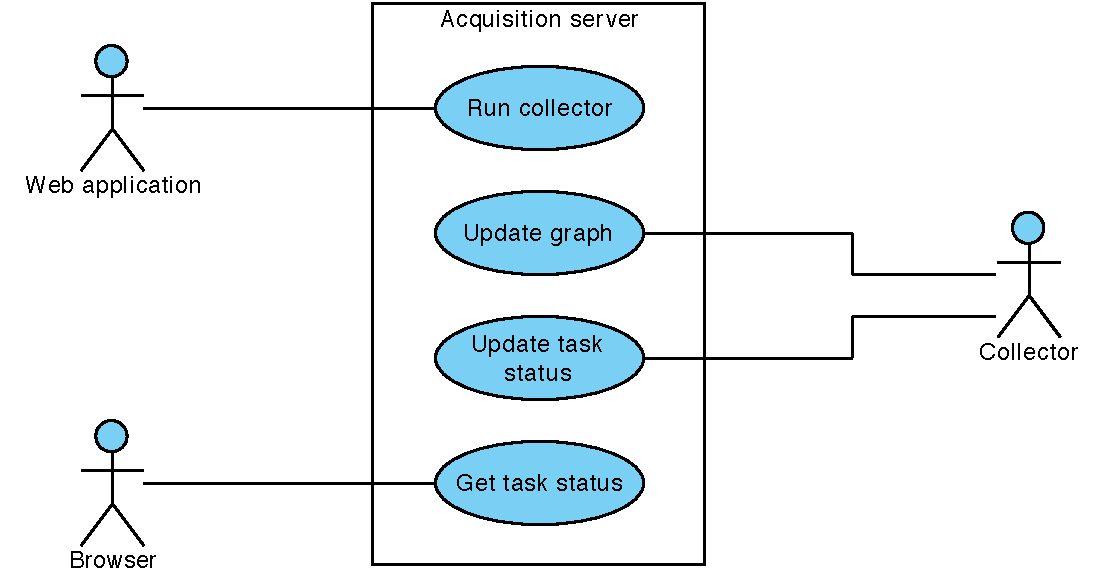
\includegraphics[width=0.75\linewidth]{images/diagrams/uc-server}
  \caption[Use case diagram for the acquisition server.]{Use case diagram from the point of view of the acquisition server.}
  \label{fig:uc-server}
\end{figure}

\begin{figure}[p]
  \centering
  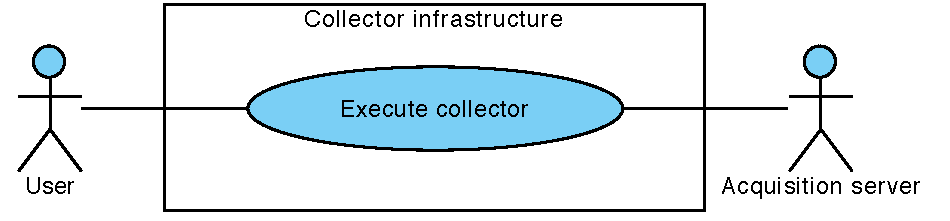
\includegraphics[width=0.67\linewidth]{images/diagrams/uc-collector}
  \caption[Use case diagram for the collector.]{Use case diagram from the point of view of the collector.}
  \label{fig:uc-collector}
\end{figure}


\subsection{Other noteworthy aspects}

\p{Introduction}
In this subsection we consider additional aspects emerged during the analysis phase worth mentioning. Some of these aspects include notes about ideas or concepts that were later discarded. In these cases, we also include a short discussion of the reasons which led us to this decision.

\p{Real-time graph construction}
Initially, we wanted the single nodes and edges to be streamed back to the web application as soon as possible, in order to be able to visualize the graph as it is being constructed. This would have a nice addition to the user interface and in some cases could also give some more insight into the data (if the acquisition timing corresponds to the historical one). However, the decision to completely decouple the acquisition and visualization modules and the important architectural overhead necessary to support this feature led us to decide to discard it.

\p{Offline and distributed processing}
By introducing the acquisition server component and making the behavior of a single controller only dependent upon its configuration, we enabled offline data acquisition sessions (the user does not need to leave his computer running, as everything is executed on the server) and laid the foundations for an easy evolution towards a more distributed architecture where each collector could be run on different computers depending on its demand in terms of resources.


\section{Design}
\label{sec:acquisition/design}


\subsection{Overview}

\p{Introduction}
In \vref{sec:case/arch} we presented the overall system architecture, composed by two main modules: the acquisition framework and the visualization application. During the analysis phase for the acquisition framework module (cf. \ref{sec:acquisition/analysis}), we further split the system down in three distinct parts: web application, acquisition server, and collector infrastructure. In this first subsection we present an overview of how the different use cases fit together sequentially, while in the successive ones we analyze each subsystem in deeper detail.

\p{Session configuration}
\Vref*{fig:seq-overview} shows a possible sequential organization of the use cases, how they are encapsulated, and which actors or systems participate in their fulfillment. The scenario presented in the figure starts with the user creating a new acquisition session, configuring it and finally configuring some collectors to fetch the actual data.

\p{Session execution}
The next logical step is to execute the acquisition session. When this use case is triggered by the user, the web application loops through each configured collector and tells the acquisition server to run each one. The acquisition server, in turn, sets up the needed infrastructure and executes each collector as a separate process.

\p{Asynchronous updating}
At this time, the acquisition session is running in the background. Each time a collector updates one of the tasks it is running, the new state is transmitted to the acquisition server by executing the \emph{Update task status} use case. This allows to keep a centralized overview of the status of all running tasks which can be queried on a per-collector basis.

\p{Checking the status of a session}
After having triggered the execution of the acquisition session, the user can display the details of the session by executing the \emph{View acquisition session} use case. When this use case is executed, the status of each collector is retrieved from the acquisition server and a new binding to receive all future updates is established. This allows a user to stay on the same web page and keep track of the execution status.

\p{Reception of new results}
Each time a collector terminates the data collection process, it updates its graph on the acquisition server, which in turn uploads it to the web application. At this moment, the page the user is viewing is updated automatically and the new results made available for viewing through the \emph{View collector graph} and \emph{View collector output} use cases.

\p{Session deletion}
Finally, if desired, the user can completely destroy all the data related to an acquisition session by executing the \emph{Delete acquisition session} use case.

\p{Subsystems design}
In the next three subsections, we analyze the three subsystems in deeper detail. The sequence diagrams related to the use cases highlighted with a thicker blue border in \vref{fig:seq-overview} are also presented in the remaining part of this section.

\begin{figure}
  \centering
  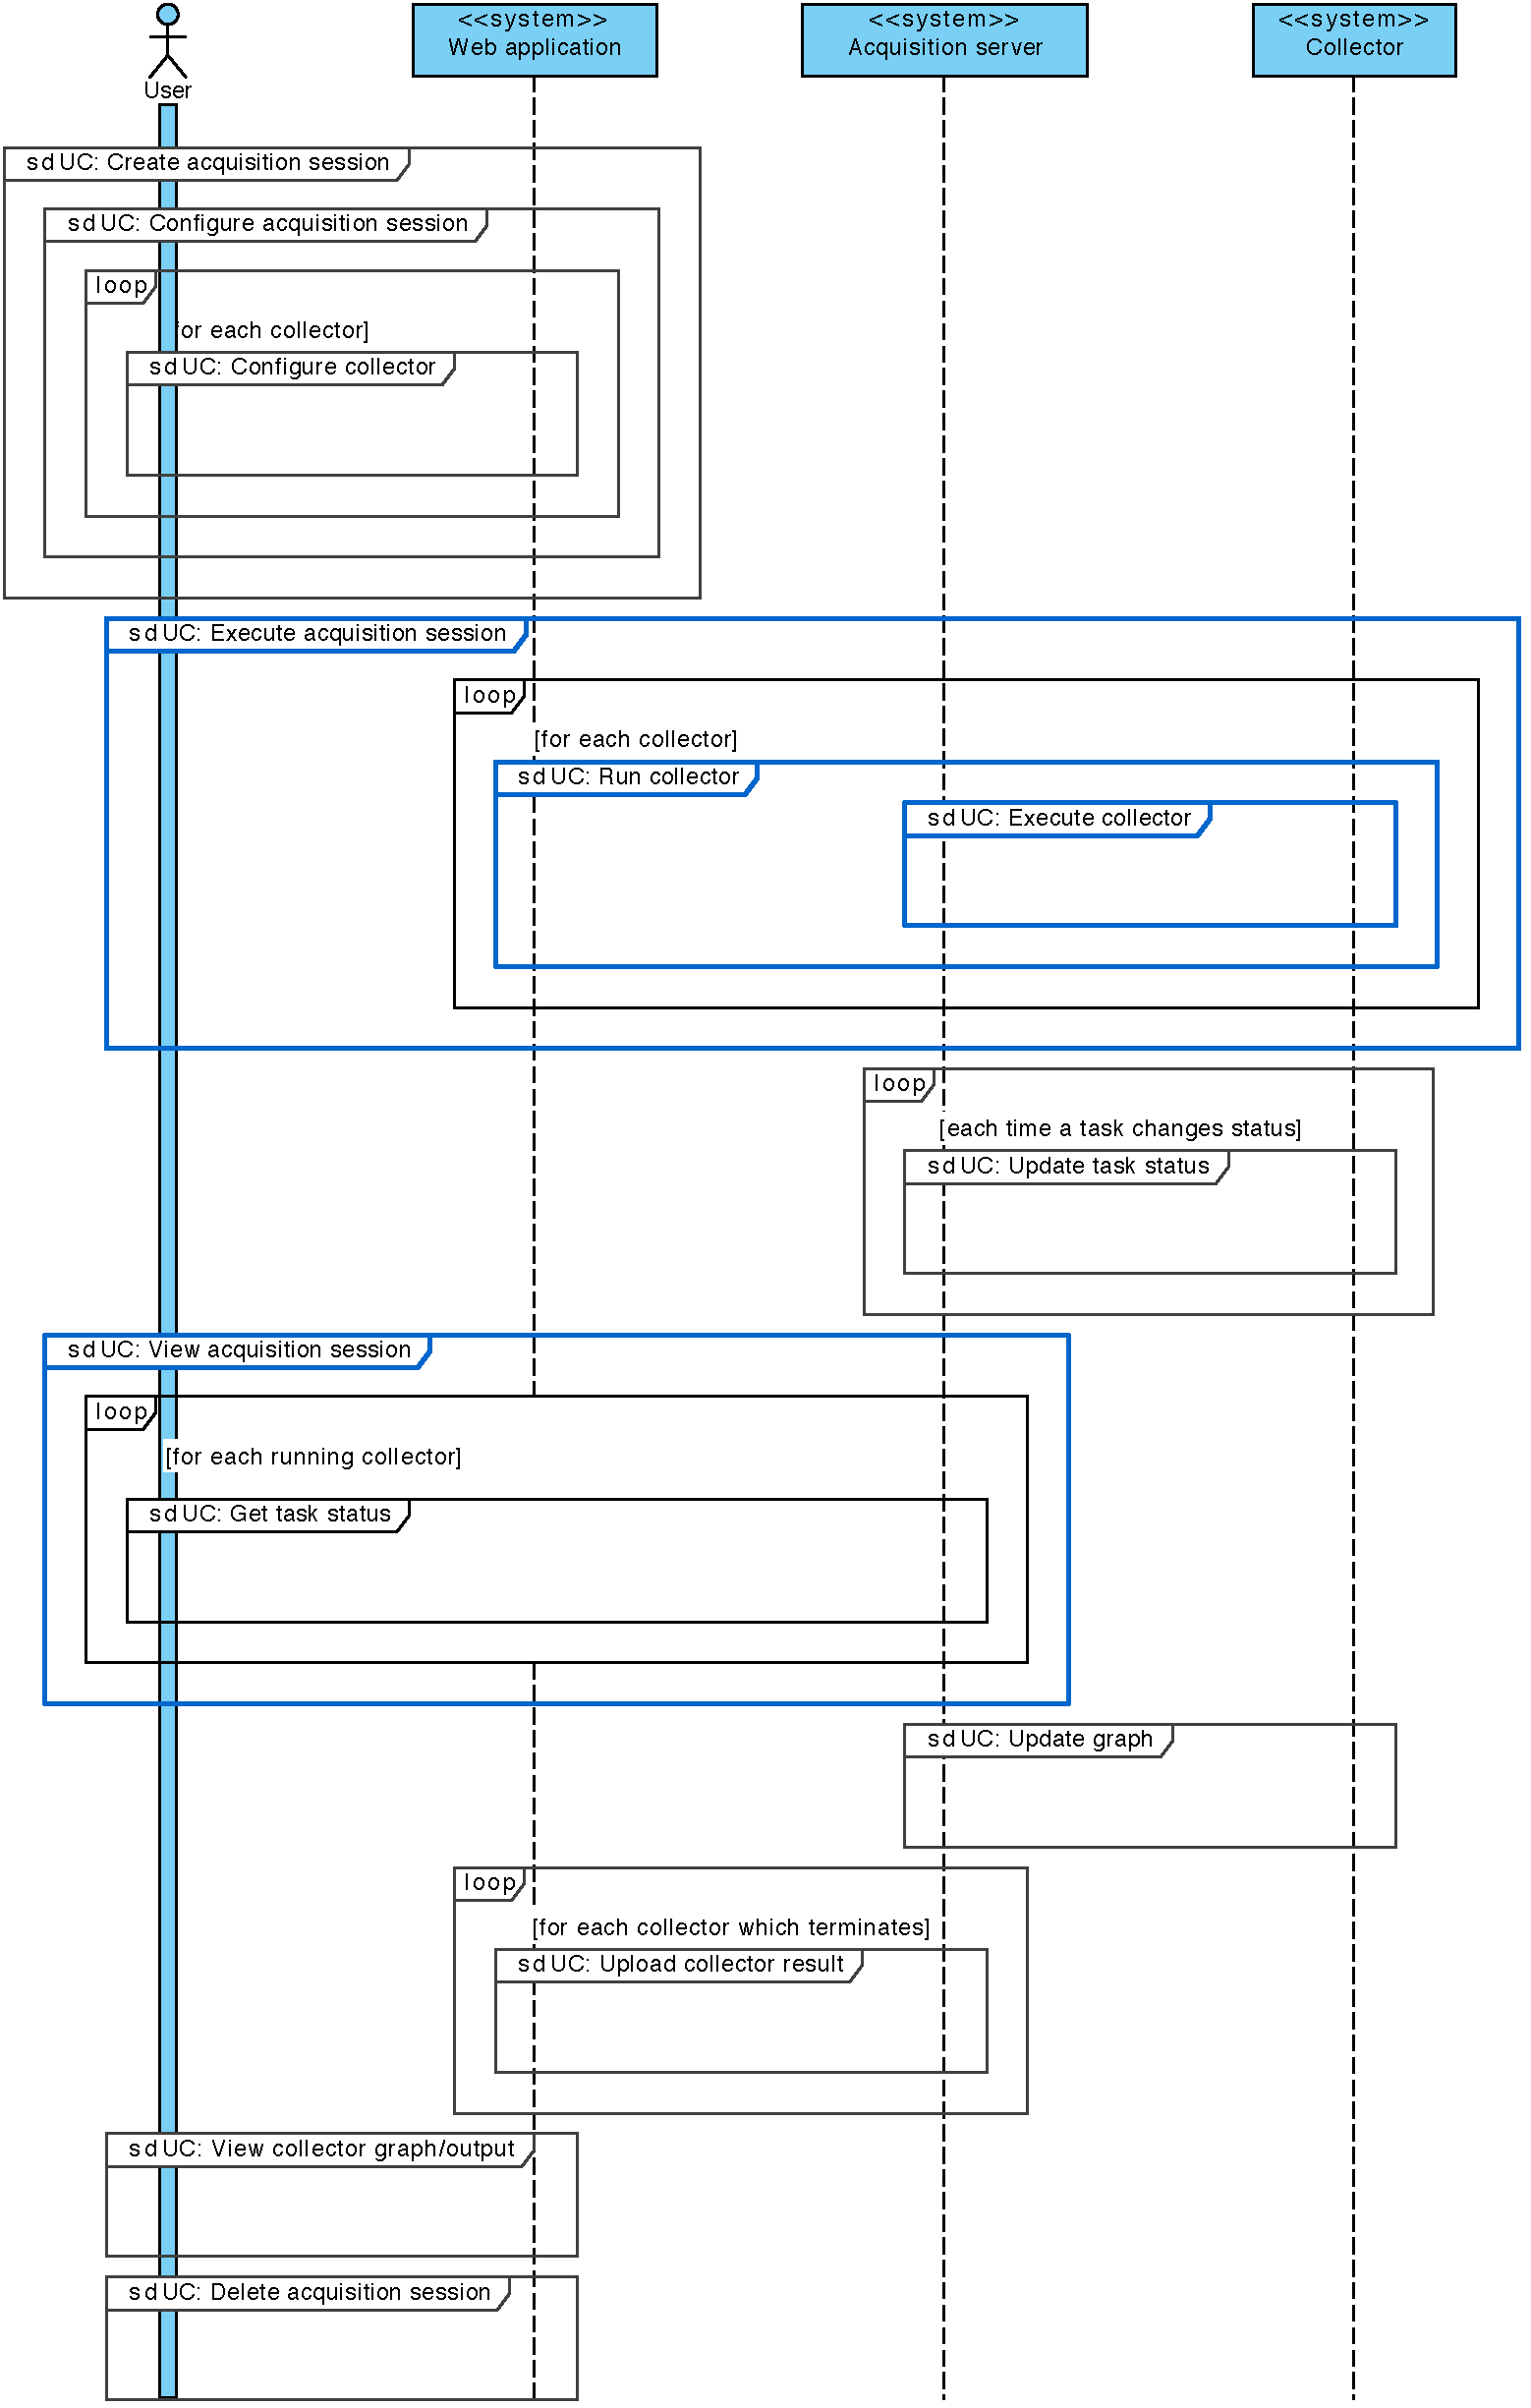
\includegraphics[width=0.95\linewidth]{images/diagrams/seq-overview}
  \caption[Overview of the mapping of the use cases to the sequence diagrams.]{Overview of the mapping of the use cases to the sequence diagrams. Use cases highlighted with a thicker border are represented in more detail in additional sequence diagrams.}
  \label{fig:seq-overview}
\end{figure}


\subsection{Web application}

\p{Introduction}
The first subsystem which we approach in greater detail is the \emph{web application}. The role of this subsystem is to expose a high-level and easy to use interface of the acquisition process to the end user. In this subsection, we will avoid to explain the design of all the \gls{crud} related operations and will instead focus on the plugin architecture to make the configuration of a range of different collector modules possible.

\p{Design scope}
As we presented in \vref{sec:case/tech}, we will use Django as MVC\footnote{Django is not a pure \gls{mvc} framework, but more something which can be described as \gls{mvt}, where the routing infrastructure along with the view represent the controller of the \gls{mvc} pattern.} framework to support the development of the web application. Django's architecture is already extensively discussed in many resources available online \cite{djangodoc} and we avoid to repeat it here. Instead we chose to focus on the system specific domain logic in a framework agnostic way.

\p{Class diagram}
To provide a better overview of how the different parts of the subsystems interact, and to show how a specific collection module can be implemented, the class diagram for the web application and the one for the collector infrastructure were grouped into a single one. The resulting diagram can be found in \vref{fig:class-collector}. As visible in the referenced figure, different classes contribute to provide the extensibility needed for the pluggable collector infrastructure.

\p{Role of the web application}
The role of the web application for the previously defined design scope is threefold:
\begin{enumerate}
  \item Provide a generic way to allow end users to configure a wide range of possibly different collectors modules. This point is addressed mainly by collector specific subclasses of \texttt{CollectorConfigForm} and \texttt{DataCollectorConfig}.
  \item Starting from the configuration defined at the previous point, being able to trigger the execution of the acquisition session by exploiting the interface offered by the acquisition server. This point is addressed by the collector specific \texttt{ICollectorConfigurator} implementation by using the data stored in the \texttt{DataCollectorConfig} instance.
  \item For each executed collector, being able to accept a resulting graph and merge those into a single one at the acquisition session level. The merging is done by the corresponding view by using the \texttt{GraphMLDocument} instance directly and saving it as an attribute of the \texttt{AcquisitionSessionConfig} instance.
\end{enumerate}
It is important to note that the web application does not have to know anything about \emph{how} a collector will be executed (or how it retrieves its data), but only \emph{which} command has to be run by the acquisition server to do so.

\p{Involved classes}
Having defined what the context and the role of the web application is, we can now delve into the description of the involved classes, some of which already introduced above. As anticipated, we will refer to the \emph{Web application} package found in \vref{fig:class-collector}.

\begin{description}
  \item[\texttt{ICollectorConfigurator}] The first entity we discuss is the \texttt{ICollectorConfigurator} interface. Classes which implement this interface are automatically recognized as data collection \emph{configuration} plugins. Their \texttt{name} attribute contains a human-readable name for the collector module, while the \texttt{key} is used internally as a unique identifier.

    Each collector configurator exposes three methods:
    \begin{description}
      \item[\texttt{get\_form\_class}] is used to retrieve the concrete \texttt{CollectorConfigForm} subclass specific to the collector implementation.
      \item[\texttt{get\_model\_class}] is used to retrieve the concrete \texttt{DataCollectorConfig} subclass specific to the collector implementation.
      \item[\texttt{run}] takes a \texttt{DataCollectorConfig} instance and executes the collector (normally by executing the \emph{Run collector} use case on the \emph{Acquisition server}).
    \end{description}
  
  \item[\texttt{ConfiguratorBase}] This abstract realization of the \texttt{ICollectorConfigurator} interface implements the default behavior of the \texttt{run} method, conforming to the sequence diagram presented in \vref{fig:seq-execute-session}. The collector-specific behavior is moved to the new abstract \texttt{get\_command} method; its task is to build the command which will be passed to the acquisition server when the \emph{Run collector} use case is executed.

  \item[\texttt{CollectorConfigForm}] This class, a concrete subclass of which is returned by the \texttt{ICollector\BreakableSlash{}Configurator.get\_form\_class} implementation, contributes to the construction of the \gls{html} form that the user will use to configure the collector in the web application. Its two methods return the two panels representing the basic and advanced configuration sets presented to the user.

    An example result of the configuration form for the \texttt{ghcomments} collector as shipped in the final release is available in \vref{fig:config-panel-example}.

  \item[\texttt{AcquisitionSessionConfig}] This class holds the generic configuration and results of an acquisition session. It is mapped to a record in the database thanks to Django's \gls{orm} and is thus persistent (as indicated by the custom stereotype, \texttt{<<ORM Persistable>>}, and yellow background). This is the only concrete class which does not need to be extended by a collector implementation.

  \item[\texttt{DataCollectorConfig}] While the configuration of the acquisition session itself is well-defined and can thus be stored in \texttt{AcquisitionSessionConfig} instances, the configuration relative to each collector depends on its implementation (e.g., the repository location for a collector which specializes in source code repository analysis). For this reason, each collector implementation also has to provide a concrete implementation of the \texttt{DataCollectorConfig} abstract class.

    The \texttt{get\_collector} method allows to get the configurator class for the specific model instance. This is needed to be able to run the collector by starting from the configuration persistently stored in the database.

    The \texttt{get\_postback\_url} method, instead, returns the unique \gls{url} which can be used by the acquisition server to upload the results of the data collection process back to the web application.

    As indicated by the stereotype and the color coding, instances of this class are persisted to the database as well.
\end{description}

\begin{figure}
  \subfloat[Basic panel]{%
		\label{fig:config-panel-basic}%
		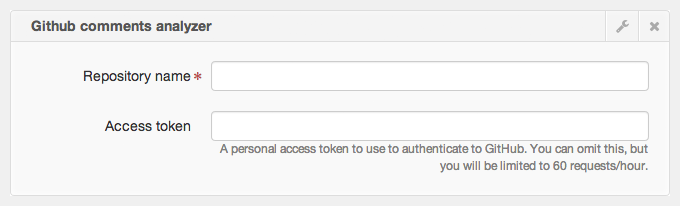
\includegraphics[height=2.43cm]{images/form-simple}
	}
	\hfill
	\subfloat[Advanced panel]{%
		\label{fig:config-panel-advanced}%
		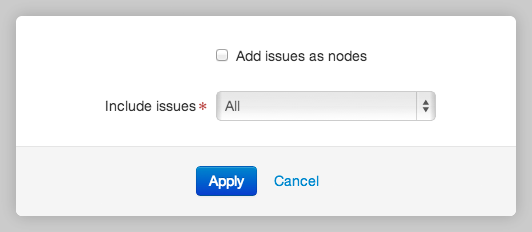
\includegraphics[height=2.43cm]{images/form-advanced}
	}
  \caption{An example of the collector configurator form for the \texttt{ghcomments} collector.}
  \label{fig:config-panel-example}
\end{figure}

\p{Sequence diagrams}
Having explained the role of each class in the package, we can now focus on their interactions and how they map to the previously introduced use cases. For this purpose, we introduce two detailed sequence diagrams: one for the \emph{Execute acquisition session} use case, in \vref{fig:seq-execute-session}, and one for the \emph{View acquisition session} use case, in \vref{fig:seq-view-session}.

\begin{figure}
  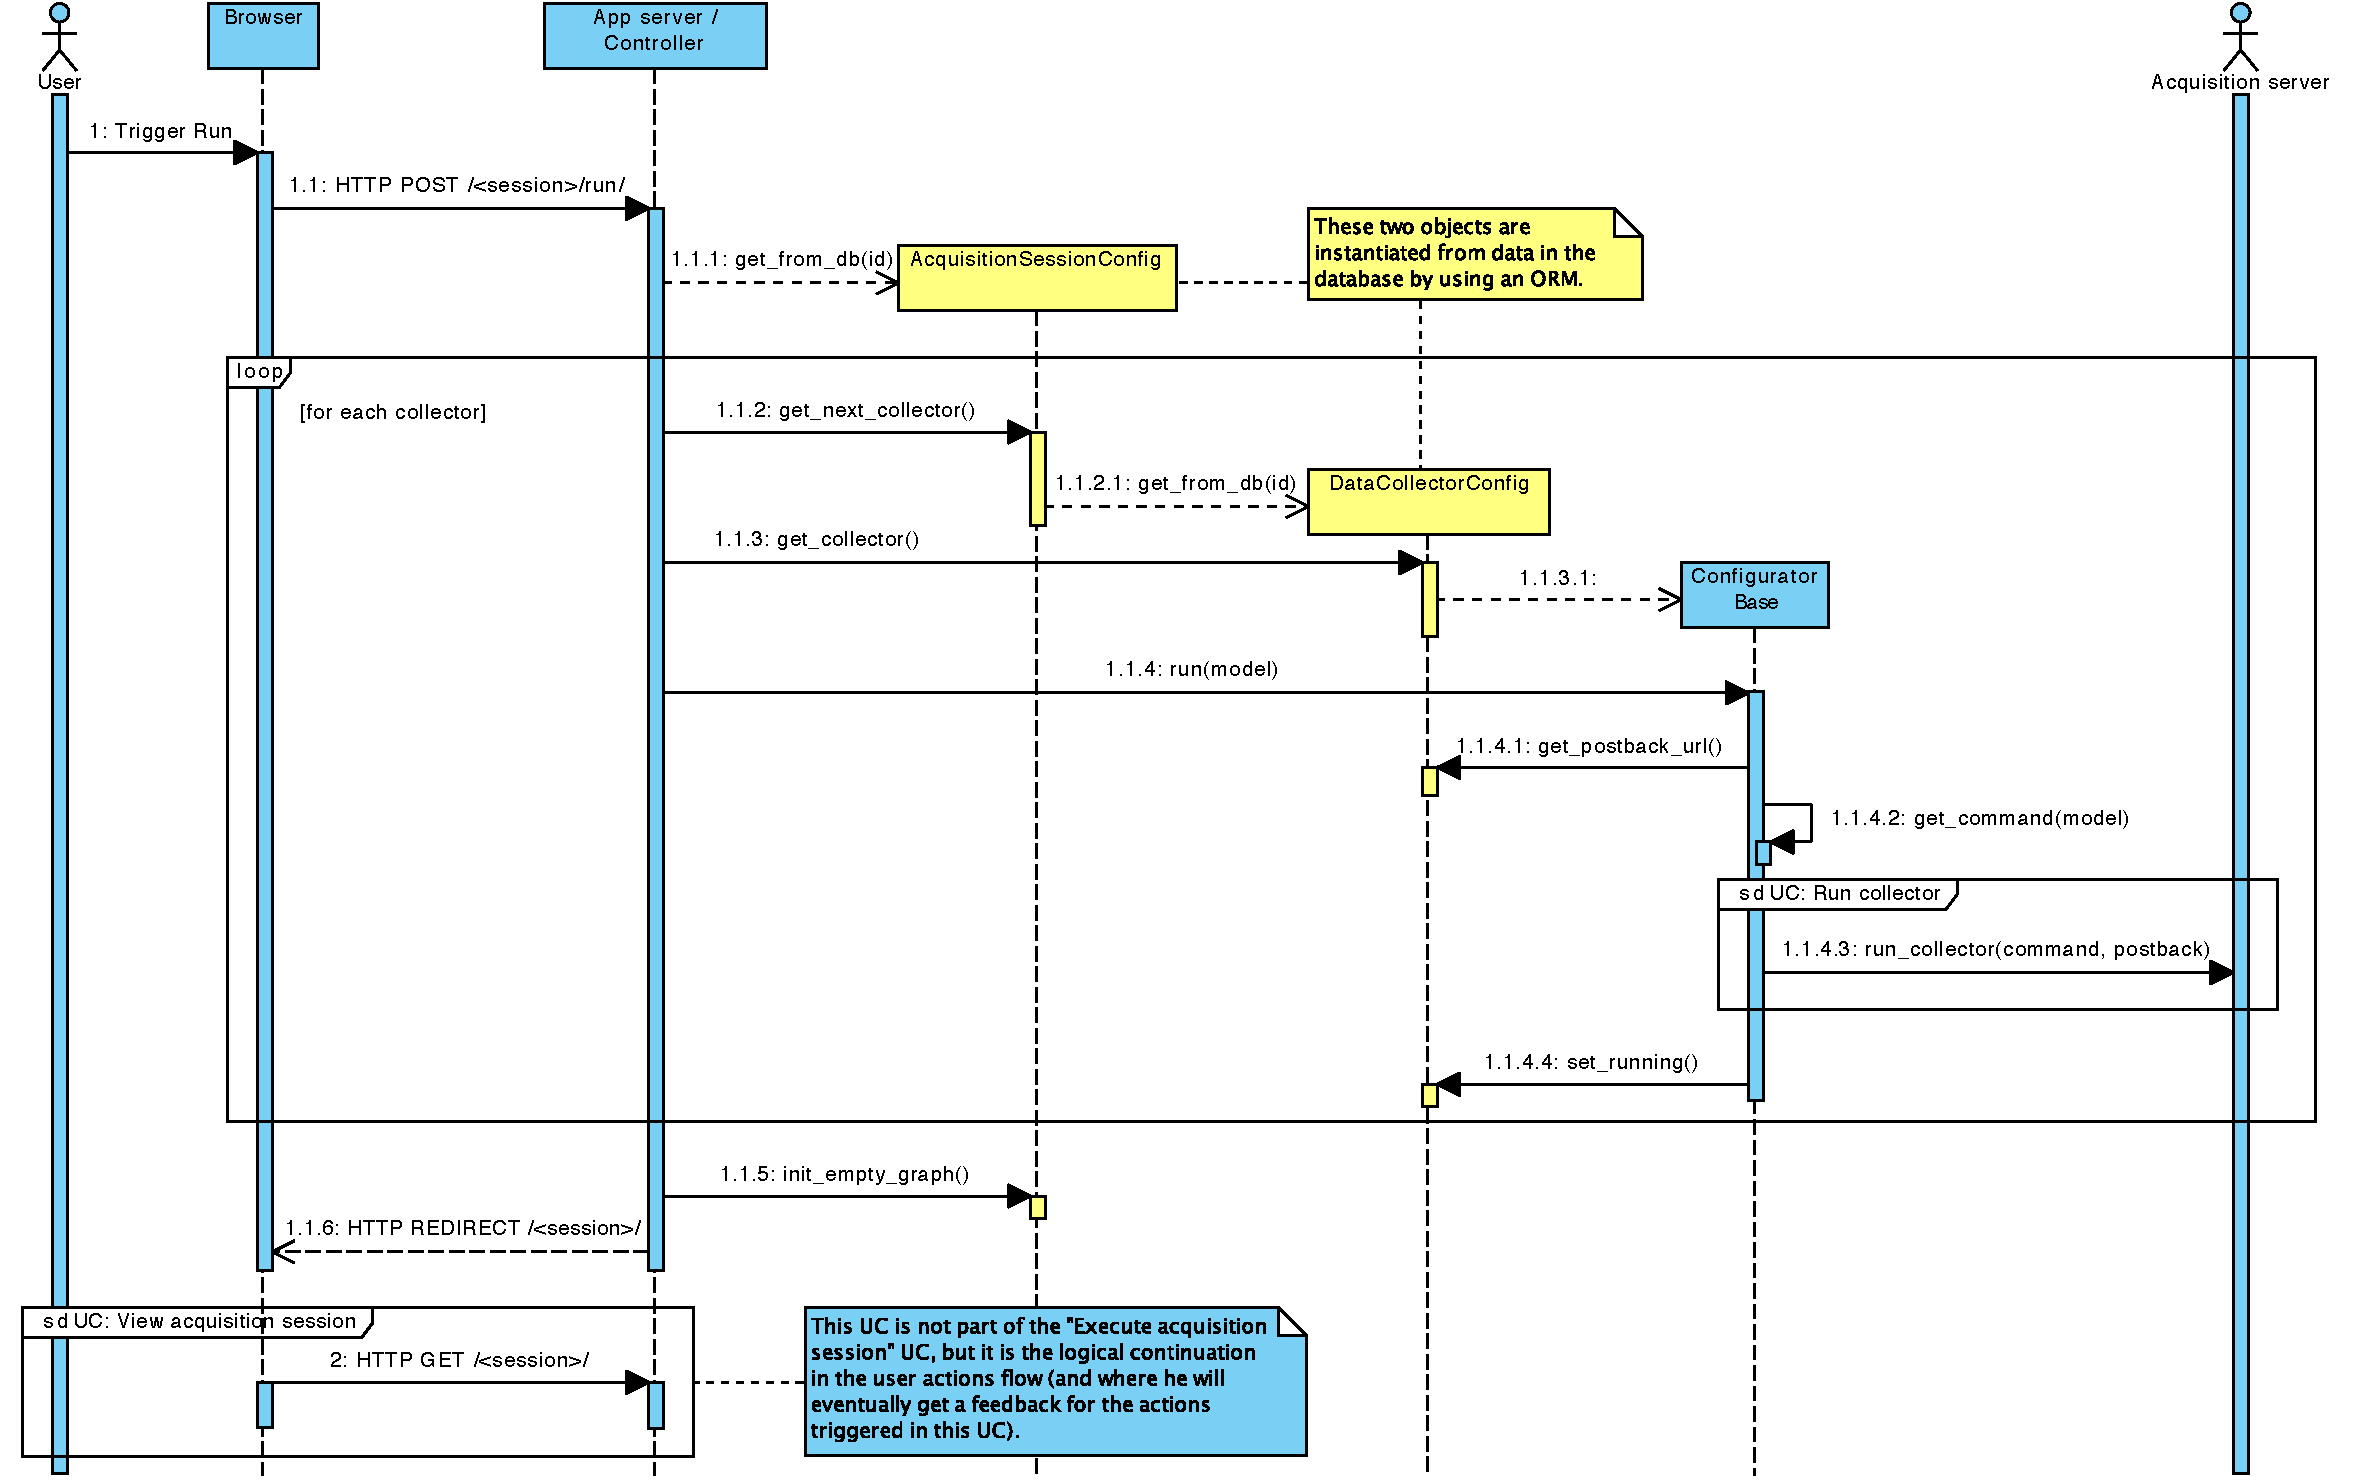
\includegraphics[height=\linewidth,angle=90,origin=c]{images/diagrams/seq-execute-session}
  \caption{Sequence diagram for the \emph{Execute acquisition session} use case.}
  \label{fig:seq-execute-session}
\end{figure}

\p{Execute acquisition session}
In the first diagram, the one for the \emph{Execute acquisition session} use case, it is visible how each collector is run starting with the retrieval of the acquisition session configuration from the database (messages 1.1.1 to 1.1.4). The diagram also gives additional details about the inner working of the \texttt{ConfiguratorBase.run} method.

\begin{figure}
  \centering
  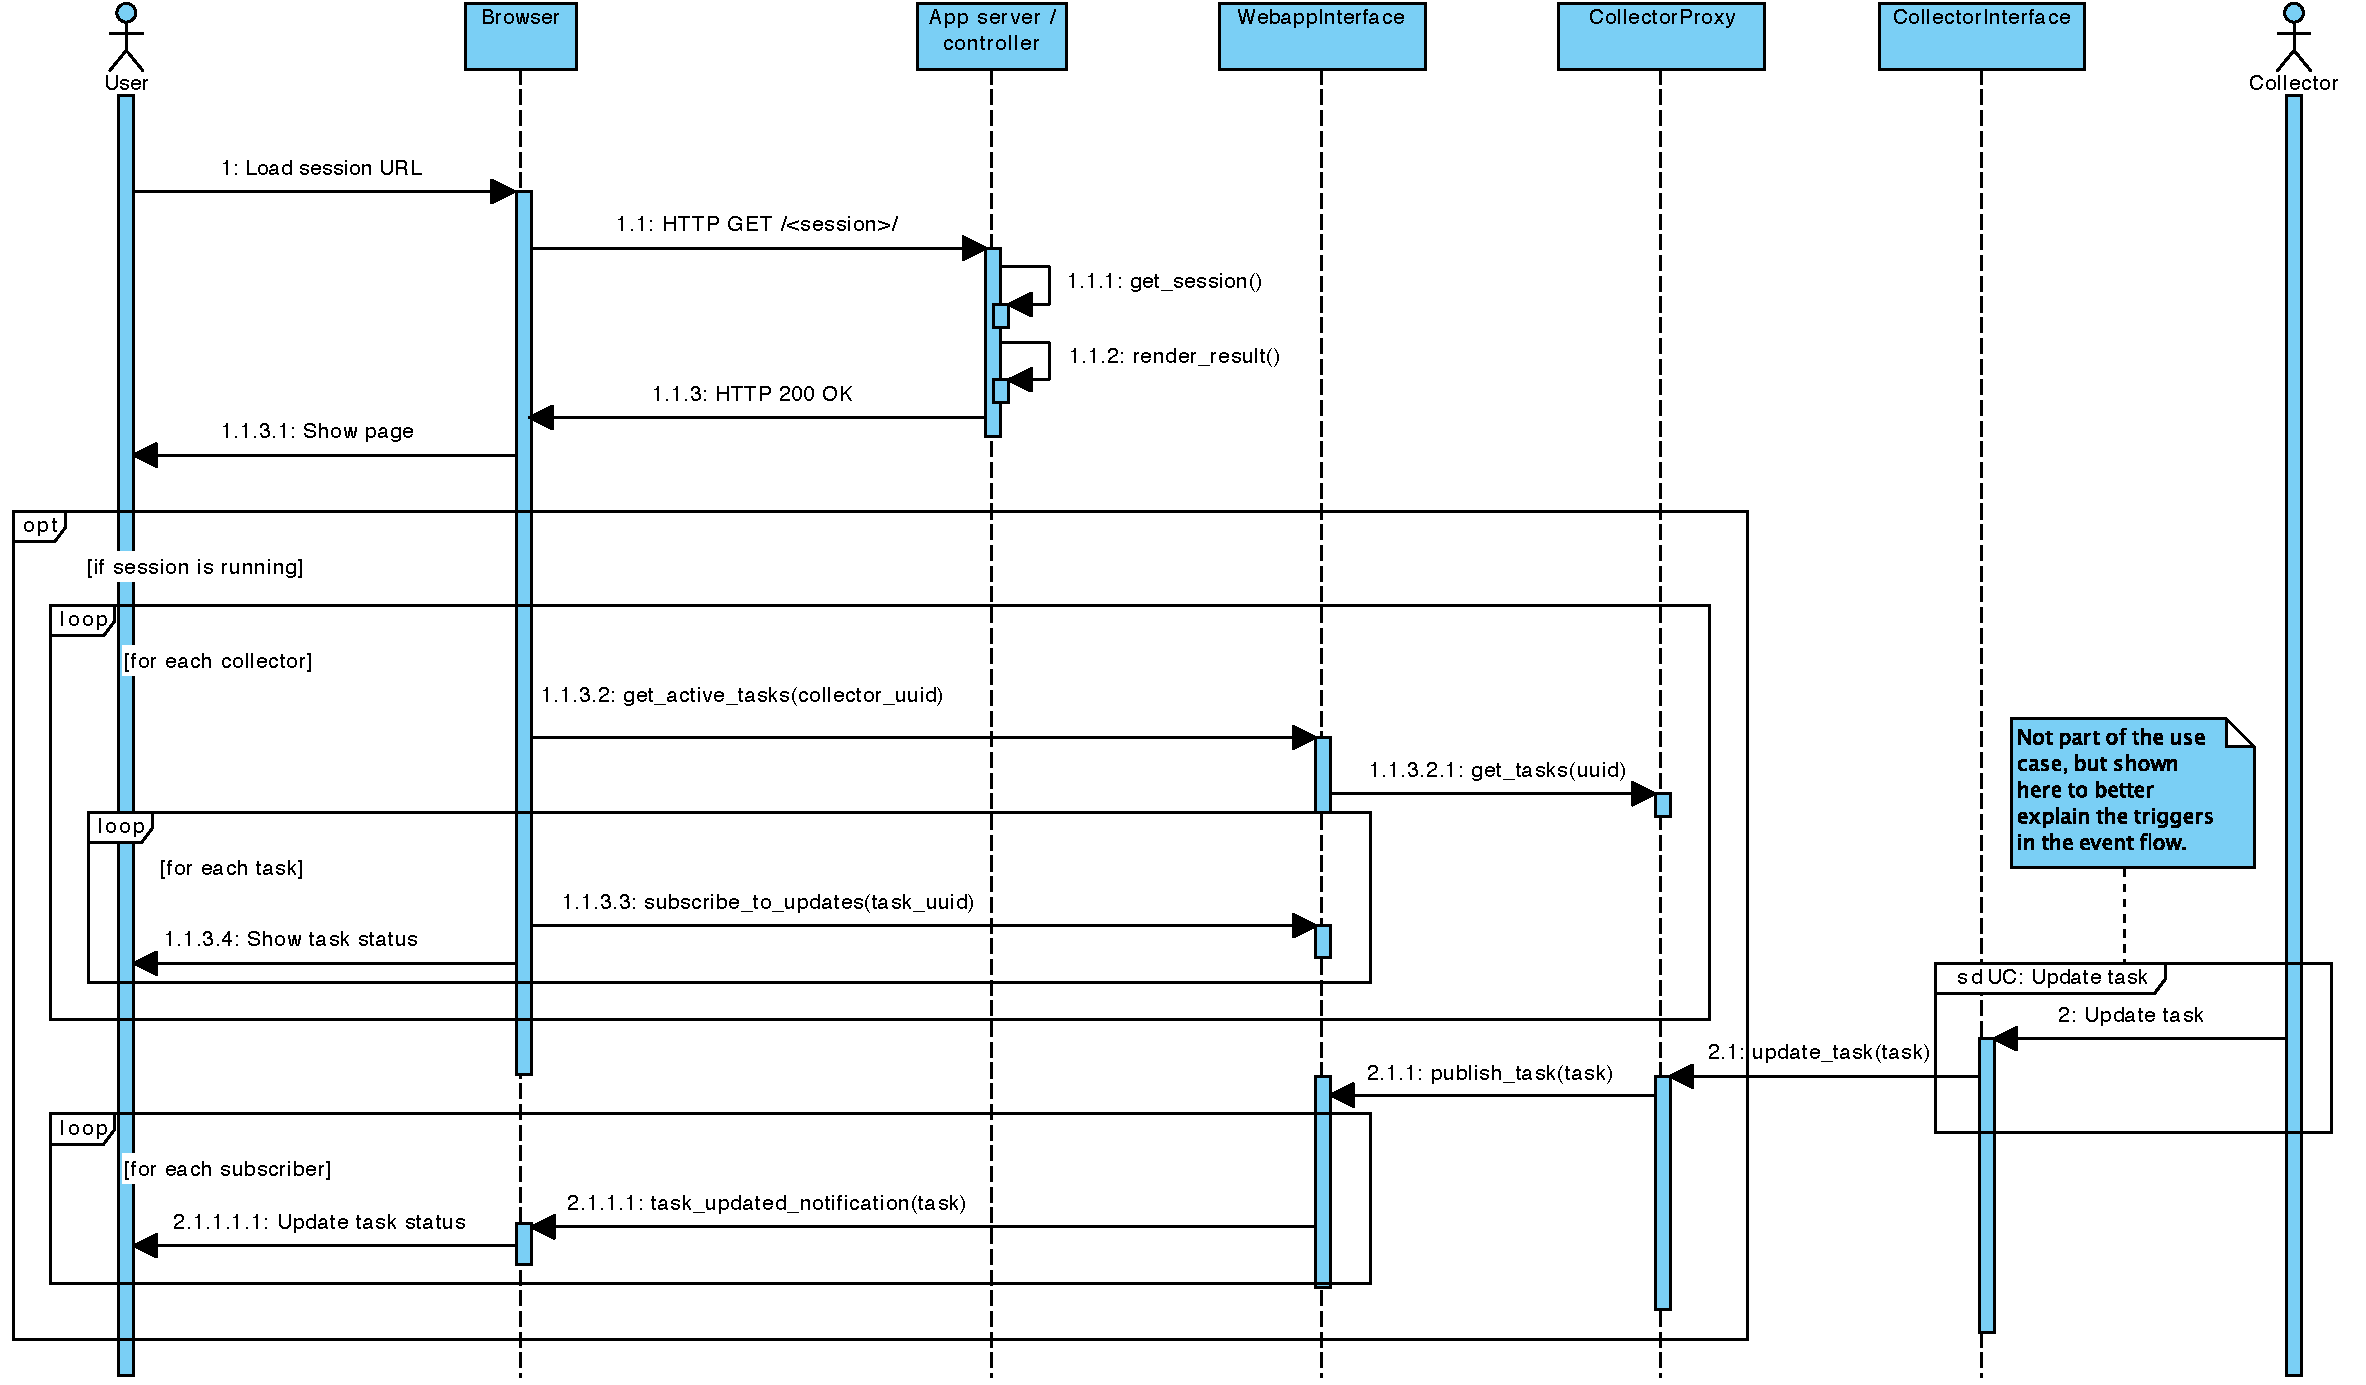
\includegraphics[height=0.95\linewidth,angle=90,origin=c]{images/diagrams/seq-view-session}
  \caption{Sequence diagram for the \emph{View acquisition session} use case.}
  \label{fig:seq-view-session}
\end{figure}

\p{View acquisition session}
The second diagram focuses on the \emph{View acquisition session} use case. The first part (messages 1 through 1.1.3.1) are a simple \texttt{GET} request to get the current acquisition session details. If the session is not running, the use case terminates here. If, instead, some collectors are still running, the browser requests their status directly to the acquisition server, without passing through the web application (messages 1.1.3.2 through 1.1.3.4). At the same time, the browser also subscribes to all future status updates. In this way, each time a collector updates a task (message 2), the information is propagated back to the user in near real-time (messages 2.1 through 2.1.1.1).

\p{Other details}
Additional details about other use cases and interactions in the web application package (for example, the implementation of the merging functionality when dealing with multiple collectors) will be presented in the corresponding subsection of the \emph{Implementation} section. In the next subsection, instead, we present the design of the acquisition server package.


\subsection{Acquisition server}
\label{sec:acquisition/design/server}

\p{Main role}
The role of the acquisition server is to accept calls to execute collectors in the form of commands, run these commands somewhere (locally or remotely) and taking care of sending the results back to the specified endpoint when the collection process terminates. Additionally, the acquisition server also provides means to keep track of the current status of all the running collectors and to provide this information on request to external entities.

\p{Scope}
Given these responsibilities, we designed the acquisition server as a networked middleware to run custom commands. In fact, beside the names of the entities, the acquisition server does not know anything about the specifics of the multi-domain data collection framework it is part of.

\p{Class diagram}
\Vref*{fig:class-collector-server} contains the class diagram for the acquisition server package. As visible thanks to the color coding, only two classes of the package are aimed to the business logic. Other parts of the system mainly contribute to provide sensible interfaces to the different actors interacting with the server. Of these, the classes belonging to the communication infrastructure (yellow background) are provided by Twisted (cf. \vref{sec:case/tech}).

\p{Exposed interfaces}
Each actor interacting with the acquisition server does so by accessing its specific interface. The web application uses the \texttt{WebappInterface} to execute collectors, the running collectors use the \texttt{CollectorInterface} to communicate updates to their tasks, while the browser uses the \texttt{Public-} and, indirectly, the \texttt{MessageBrokerInterface} to get and subscribe to the task statuses, respectively.

\p{Communication protocols}
All communication between the acquisition server and the interacting entities use the \texttt{JSON-RPC} protocol \cite{jsonrpc}. The support to encode/decode method calls using this protocol is provided by the \texttt{JsonRpcProtocol} class. While \texttt{JSON-RPC}-encoded data can be transferred over a raw \gls{tcp} connection, only the web application does so. To allow for bidirectional push operations, the browser encapsulates the \texttt{JSON-RPC} payload in a \emph{Websocket} \cite{websocket} connection. This is made possible on the acquisition server side by exposing the \texttt{PublicInterface} instance encapsulated in a \texttt{WebsocketProtocol} instance. The collectors, on the other hand, do not communicate with the acquisition server over the network but simply by writing directly to their standard output streams. These streams are piped to a \texttt{ProcessProtocol} instance, which, in turn, writes the received data to the \texttt{CollectorInterface} instance.

\p{Business logic}
The remaining two classes in the package, \texttt{AcquisitionServer} and \texttt{CollectionProxy}, wrap the business logic. \texttt{AcquisitionServer} gets instantiated when the server is started and acts as the central controller. Each time a collector has to be run, it creates a new \texttt{CollectorProxy} instance, returns its identifier to the calling entity and then, asynchronously, invokes the \texttt{CollectorProxy.run} method. This behavior is shown graphically in the sequence diagram in \vref{fig:seq-run-collector}.

\p{Other details}
The remaining classes, outside the \emph{Acquisition server} package, provide general-purpose infrastructure, namely a simple message broker to route messages from specific collectors to their listeners, and the task management functionalities needed to the bookkeeping of the different tasks the collectors are running.

\begin{figure}
  \centering
  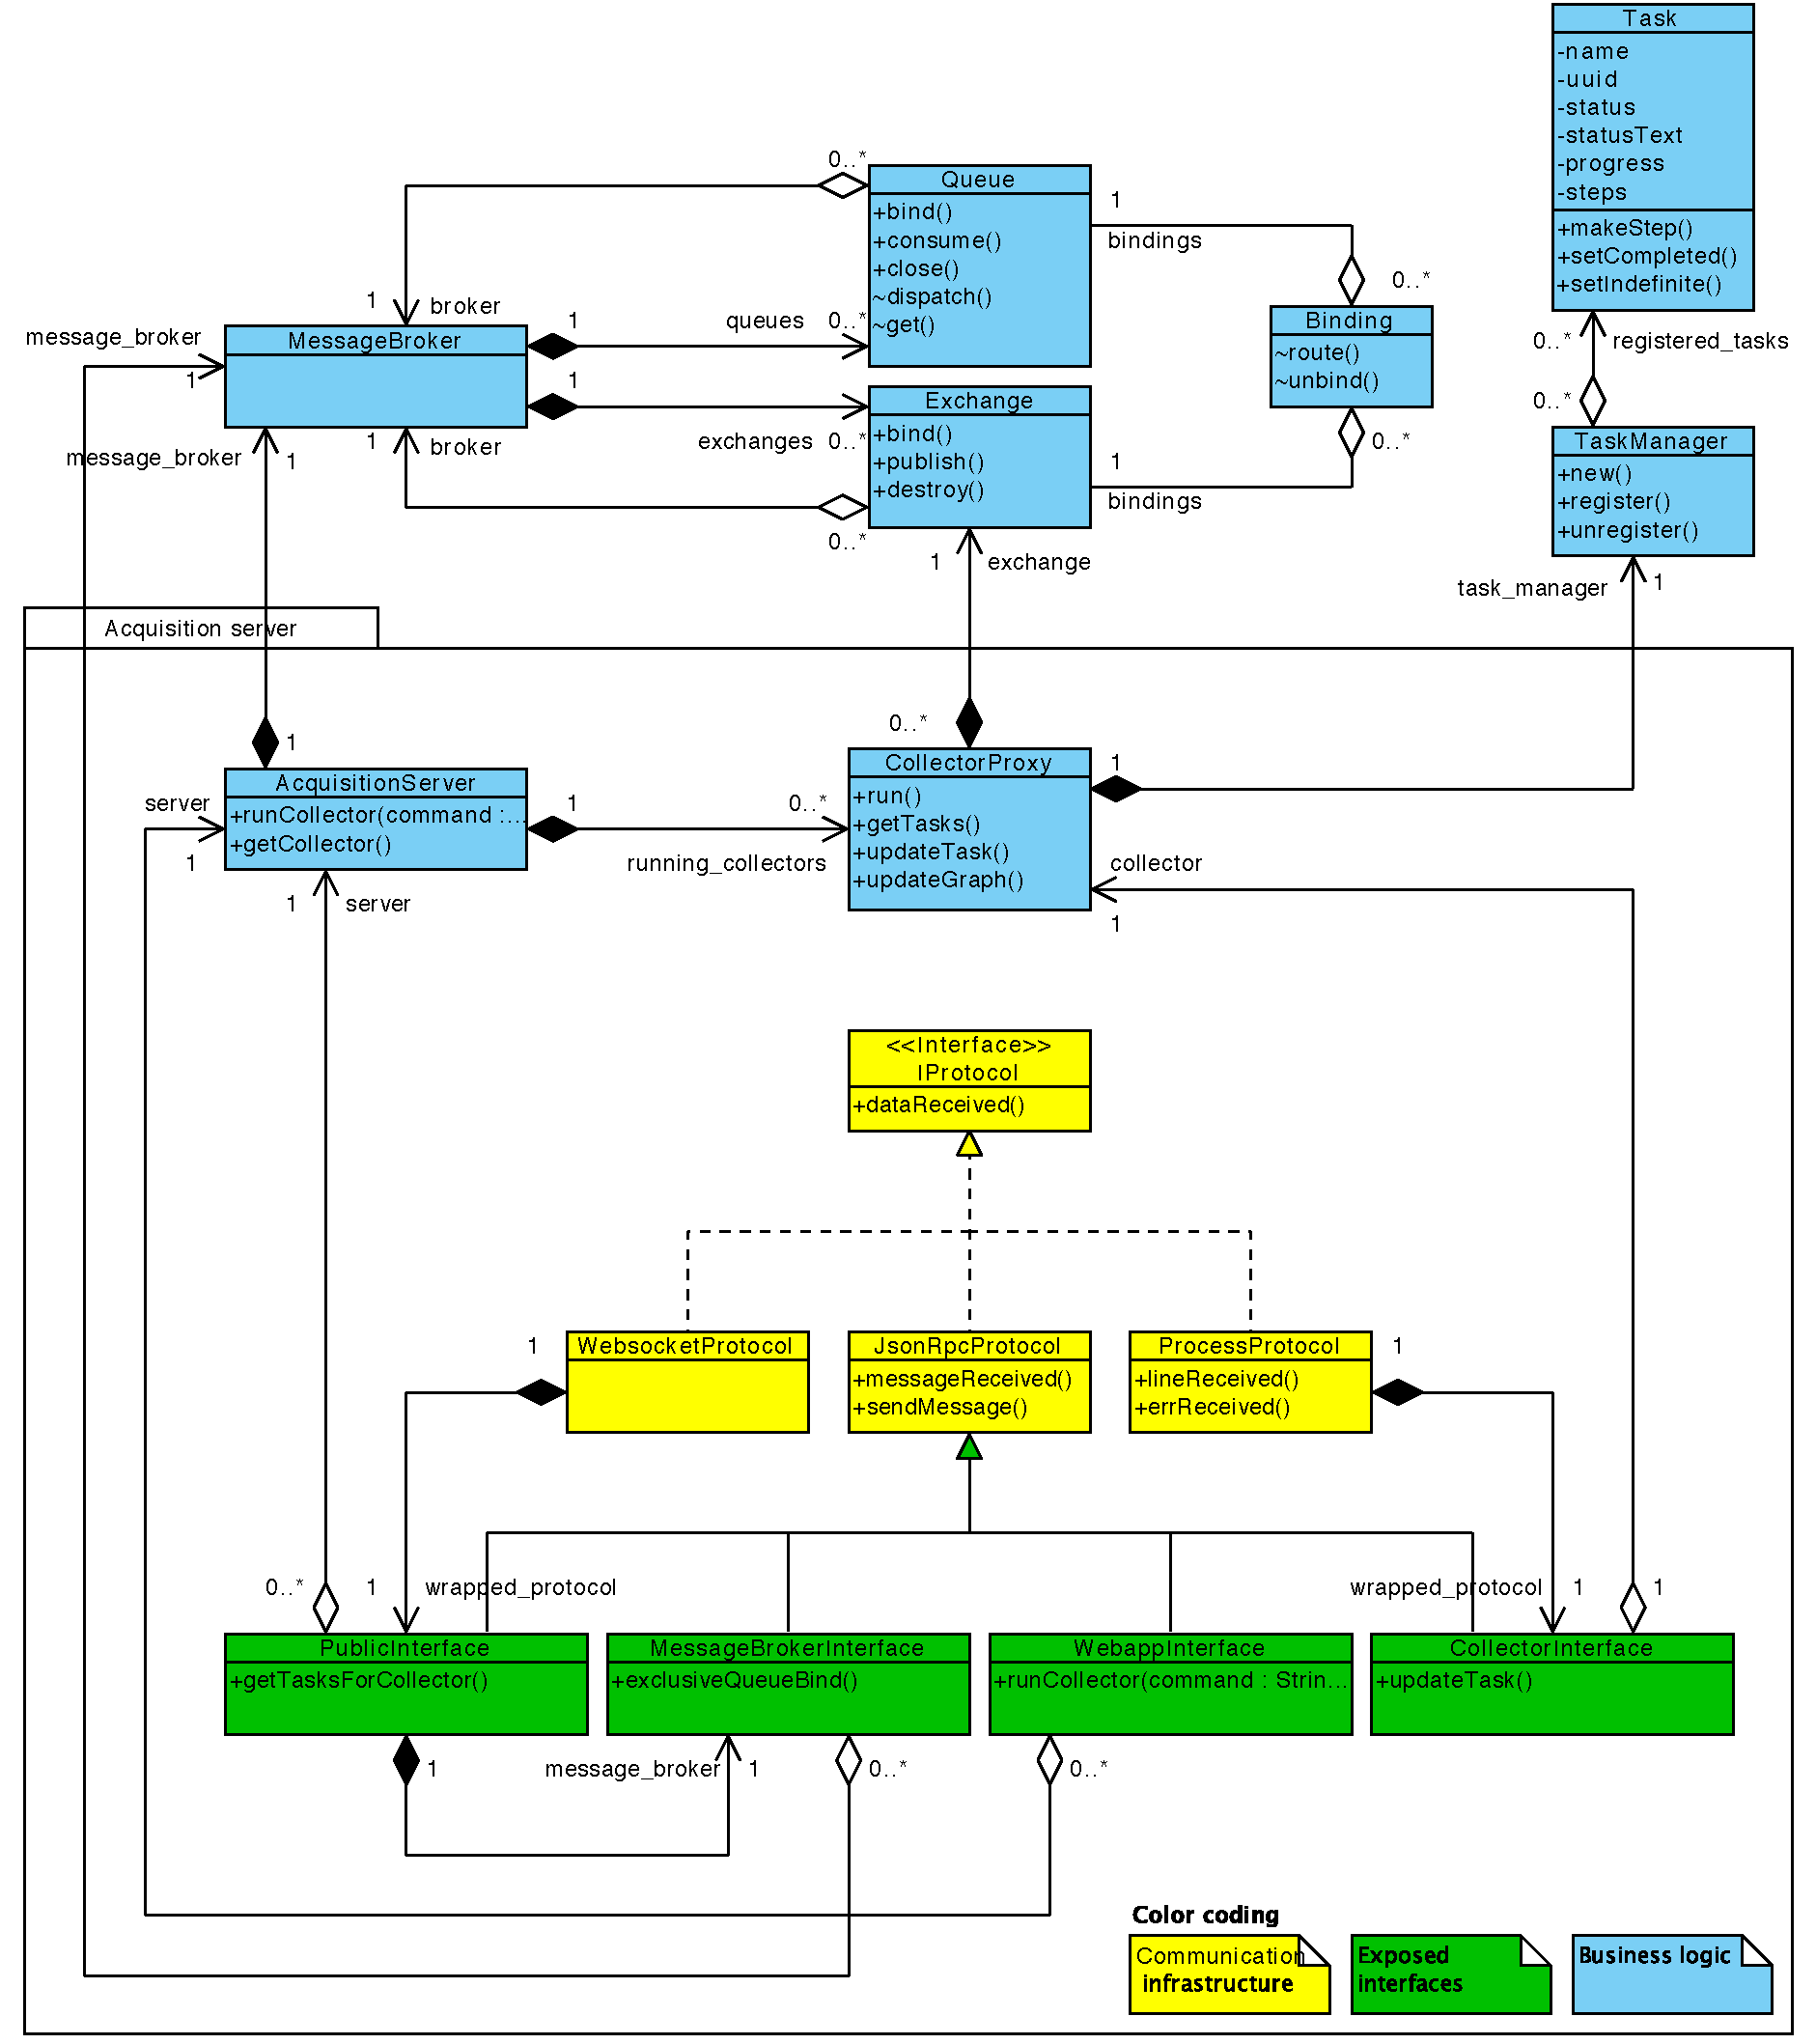
\includegraphics[width=0.98\linewidth]{images/diagrams/class-collector-server}
  \caption[Class diagram for the acquisition server.]{Class diagram for the acquisition server.}
  \label{fig:class-collector-server}
  \vspace{1cm}
\end{figure}

\begin{figure}
  \begin{adjustwidth}{-7.5mm}{-1.5cm}
    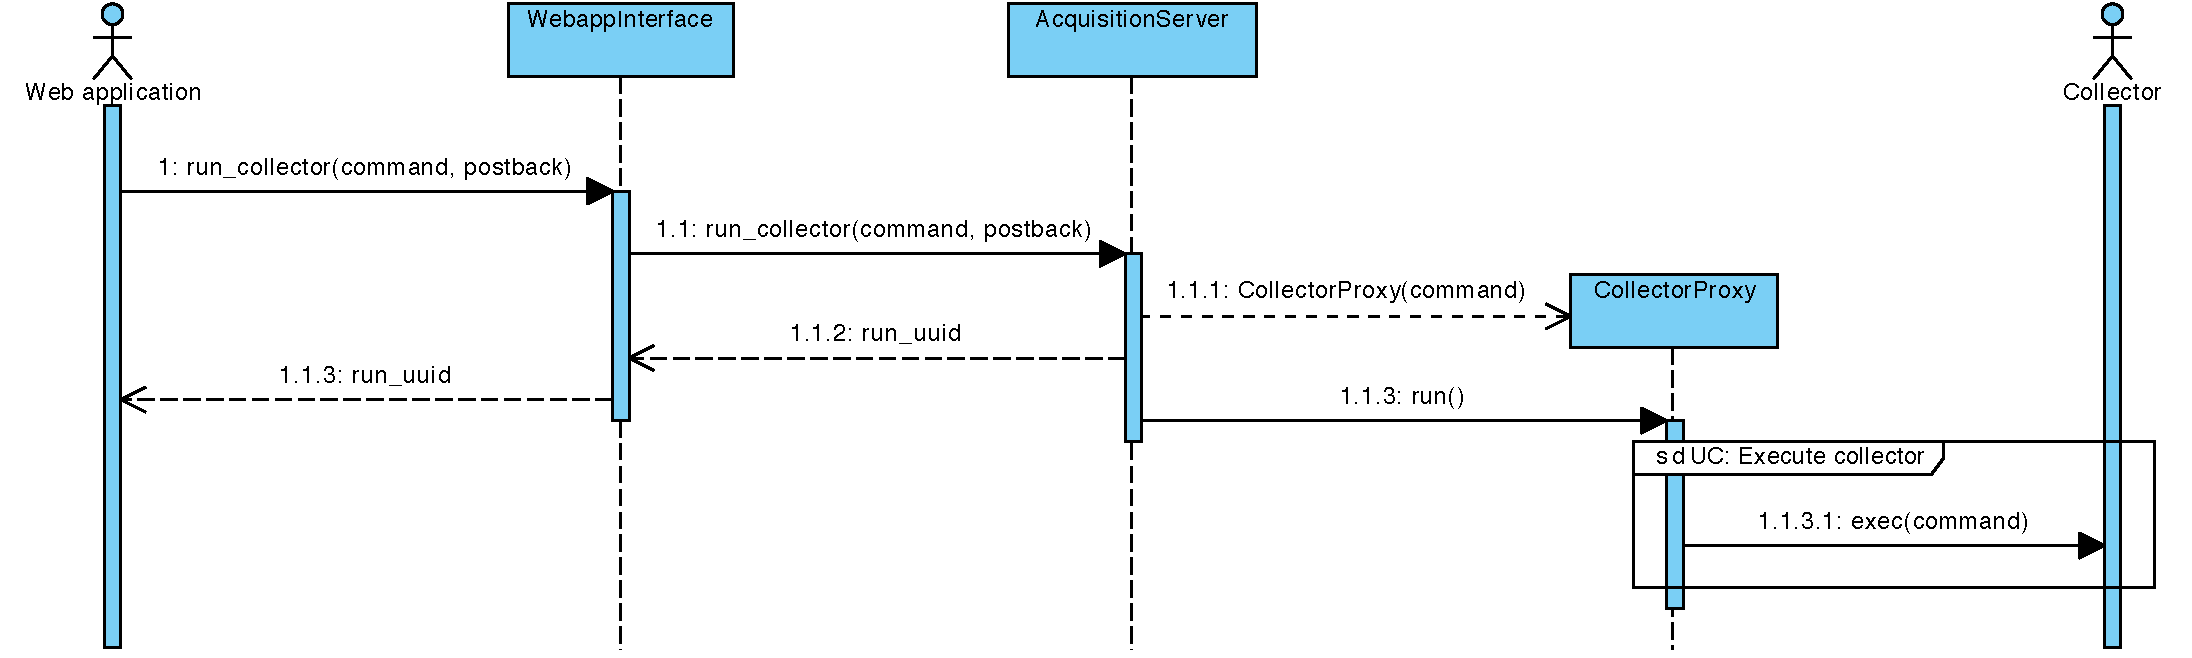
\includegraphics[width=\linewidth]{images/diagrams/seq-run-collector}
  \end{adjustwidth}
  \caption{Sequence diagram for the \emph{Run collector} use case.}
  \label{fig:seq-run-collector}
\end{figure}


\subsection{Collector infrastructure}

\p{Introduction}
The last subsystem for which we present the design is the collector infrastructure. This subsystem plays a central role in the data acquisition process. In fact, it is possible to collect data by using the collector infrastructure uniquely instead of dealing with the web application and, indirectly, via the acquisition server.

\p{Role}
The role of the collector infrastructure is to provide a complete set of hooks and utilities to ease the development and integration of custom data collection modules. Thanks to these classes, the module developer can focus completely on the domain-specific data-retrieval logic, while all the heavy lifting (invocation, task management, graph creation, \ldots) is already taken care of.

\p{Class diagram}
\Vref*{fig:class-collector}, already introduced in the presentation of the web application design, contains the class diagram for the collector infrastructure package. The classes contained therein can be described in the following way:

\begin{description}
  \item[\texttt{RunnerBase}] When executed, the collector infrastructure instantiates one of the two \texttt{Runner\BreakableSlash{}Base} subclasses; either \texttt{ConsoleRunner} if the collector was invoked manually from the command line, or \texttt{RemoteRunner} if the collector was invoked from the acquisition server. The \texttt{RunnerBase} class is responsible for parsing the argument, creating a task manager, delegating the creation of the module specific \texttt{ICollectorImplementation} to the \texttt{ICollectorFactory}, and executing the collector.

    The two subclasses simply provide a specialized \texttt{TaskManager} subclass, one which writes the task status to the standard output in human-readable form (\texttt{ConsoleTask\BreakableSlash{}Manager}) and one which outputs \texttt{JSON-RPC}-encoded method calls (\texttt{RemoteTask\BreakableSlash{}Manager}) intended for the acquisition server.
  \item[\texttt{ICollectorFactory}] Custom data collection modules have to provide a realization of this interface in order to be discovered by the system and be added to the data collectors registry. The \texttt{name}, \texttt{key} and \texttt{version} attributes are the same as for the \texttt{ICollector\BreakableSlash{}Configurator} already presented in the web application design subsection. The additional two methods can be described as follows:
    \begin{description}
      \item[\texttt{build\_parser}] is responsible to parse the command line into collector specific arguments in order to allow to expose a unified command line interface across all installed collector modules.
      \item[\texttt{build\_collector}] takes the parsed arguments and returns a configured instance of the module specific \texttt{ICollectorImplementation} realization.
    \end{description}
  \item[\texttt{FactoryBase}] This abstract \texttt{ICollectorFactory} realization implements a basic version of the \texttt{build\_parser} method which can optionally be overridden by the subclass.
  \item[\texttt{ICollectorImplementation}] A module specific instance of a realization of this interface is returned by the collector factory upon request by the runner. Its only required method, \texttt{run}, is responsible to execute the data collection process and return a \texttt{GraphMLDocument} instance.
\end{description}

\begin{figure}[p] 
  \centering
  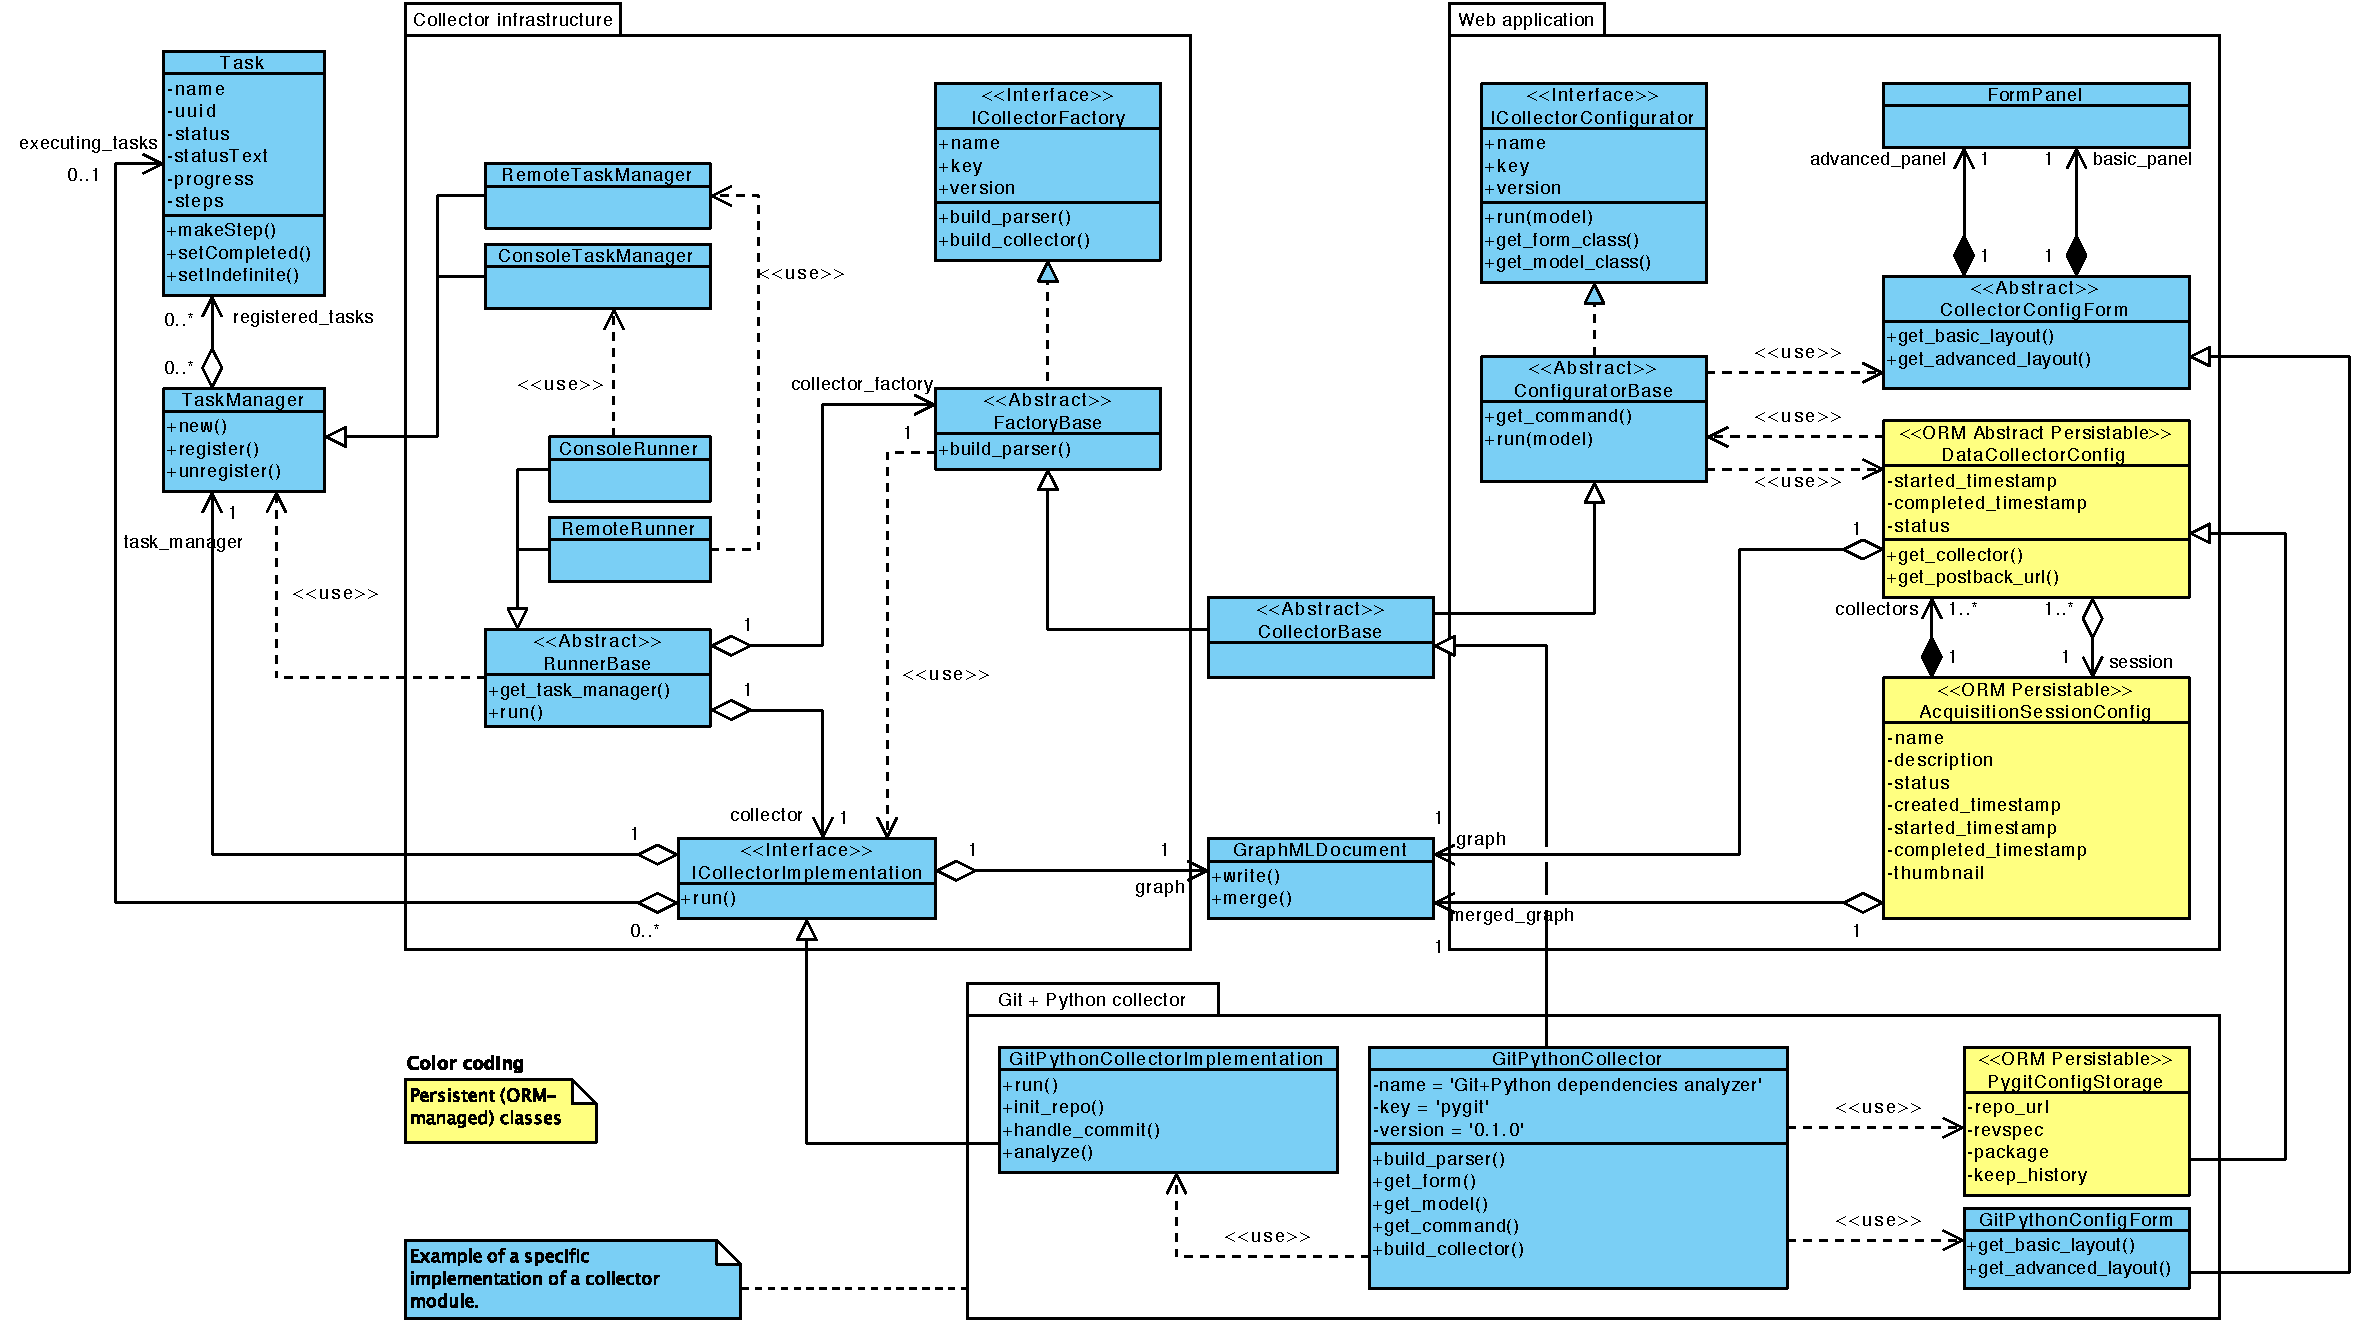
\includegraphics[height=0.93\linewidth,angle=90,origin=c]{images/diagrams/class-collector}
  \caption[Class diagram for the data collection infrastructure.]{Class diagram for the collector infrastructure and the web application used to manage it.}
  \label{fig:class-collector}
\end{figure}

\p{Sequence diagram}
The sequence diagram presented in \vref{fig:seq-execute-collector} illustrates how the different presented components interact to fulfill the \emph{Execute collector} use case. The user or the acquisition server command is passed to the correct \texttt{Runner\BreakableSlash{}Base} subclass (message 1) which in turn parses it (messages 1.1 and 1.2), instantiates the required \texttt{TaskManager} subclass (message 1.3 and 1.3.1) and asks the factory to build the collector implementation instance (message 2). At this point all required components are ready and the data collection can be launched (message 3). Once the control of the execution flow is passed to the collector, the collector itself creates the tasks it needs to fulfill its job and, after the data was collected, returns the graph representing it to the runner. Before exiting, the runner writes the graph to its standard output by executing the \emph{Update graph} use case (messages 4 and 4.1).

\begin{figure}
  \begin{adjustwidth}{-11.6mm}{-2cm}
    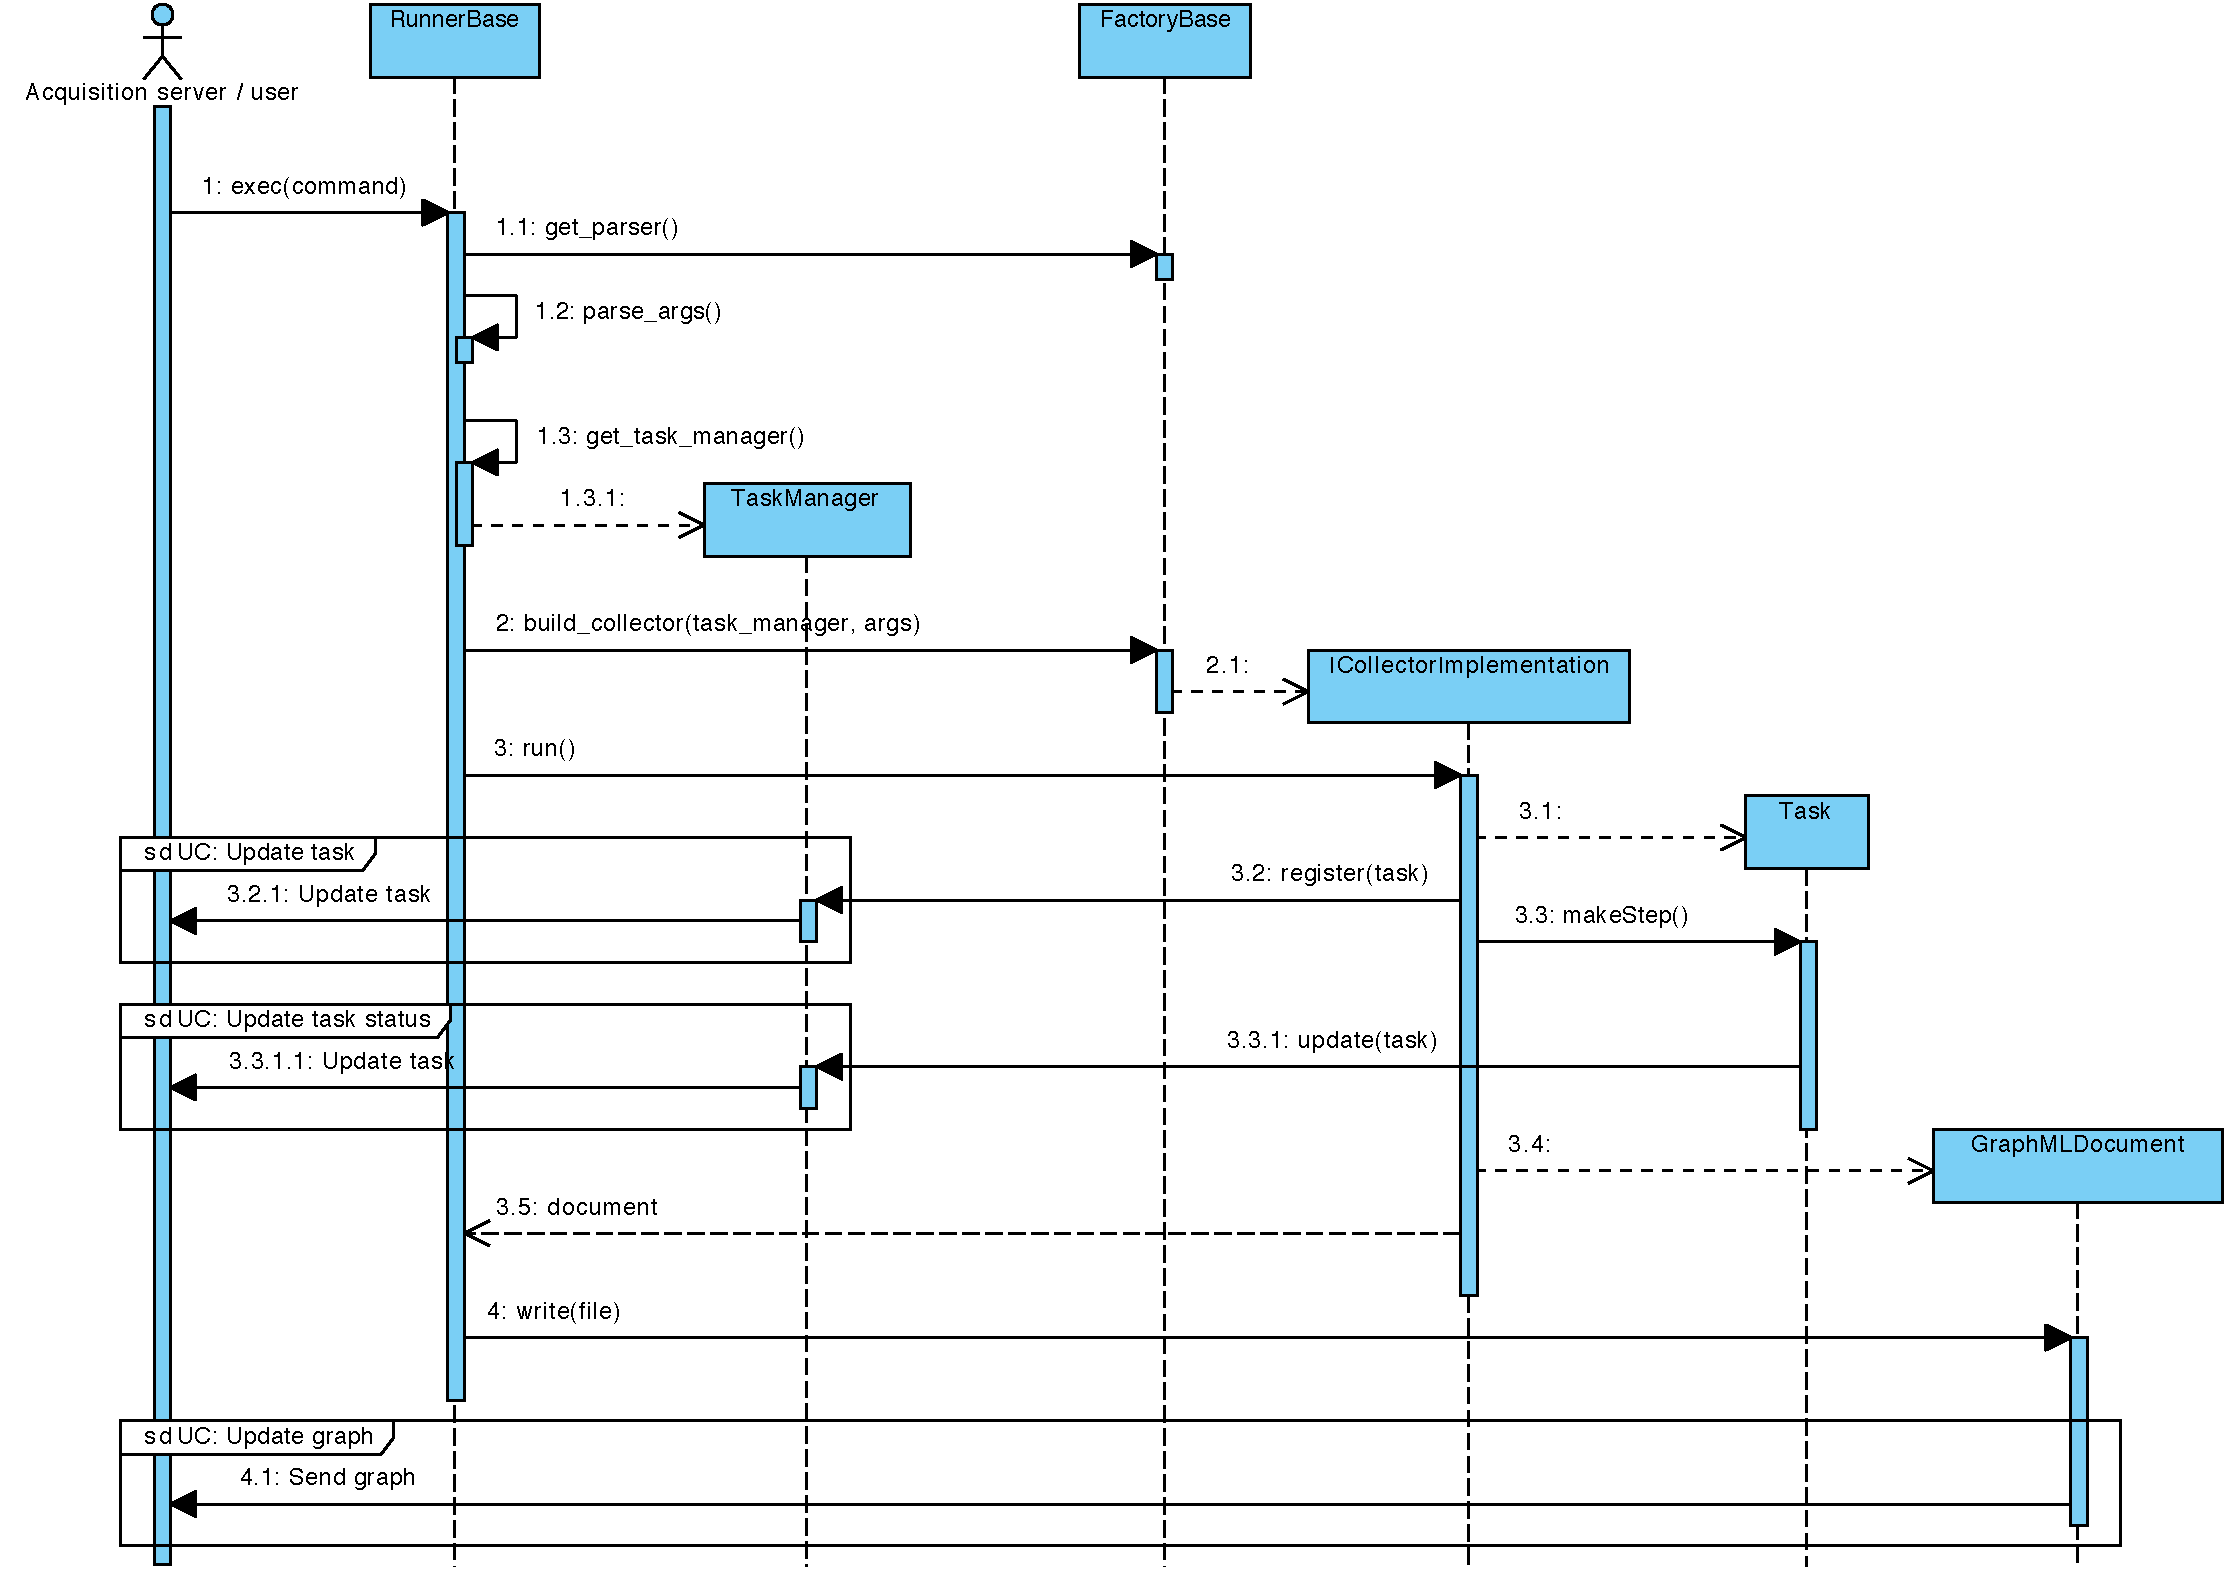
\includegraphics[width=\linewidth]{images/diagrams/seq-execute-collector}
  \end{adjustwidth}
  \caption{Sequence diagram for the \emph{Execute collector} use case.}
  \label{fig:seq-execute-collector}
\end{figure}

\p{Conclusions}
In the current section we presented a highly modular design for the data acquisition framework. The goal of the presented architecture is to enable developers to easily write custom acquisition modules while focusing only on the data collection logic. In the next section we present how this design was brought into reality by highlighting interesting aspects of its implementation. Finally, in the last section, we describe some of the results of this particular infrastructure by introducing different, domain-specific, data acquisition modules.

\section{Implementation}
\label{sec:acquisition/implementation}

\p{Introduction}
In the present section we discuss interesting problems and their solutions occurred during the implementation of the previously discussed design. During the analysis and design phases, we approached the system as a set of three completely decoupled entities. While this decoupling is reflected in the implementation as well, we structured the present section by feature instead of system. The reason behind this decision is that most discussed points concern more than one subsystem at once and are thus best approached in an integrated way.

\subsection{Plugin registration and discovery}

\p{Plugin discovery}
One of the main selling points of the whole acquisition framework is its pluggable architecture. Custom data acquisition modules can be built by implementing the exposed interfaces and they will automatically be integrated in the application. We exploit Twisted's plugin system to discover and register the custom acquisition modules with the system. The discovery step is easily addressed by the \texttt{get\_collectors} and \texttt{get\_factories} functions shown in \vref{lst:plugin-discovery}.

\begin{lstlisting}[caption={Custom acquisition modules discovery.},label=lst:plugin-discovery]
from twisted import plugin
from csat import collectors
from csat.acquisition import base

def get_collectors():
    return plugin.getPlugins(base.ICollectorConfigurator, collectors)

def get_factories():
    return plugin.getPlugins(base.ICollectorFactory, collectors)
\end{lstlisting}

\p{Plugin registration}
The discovery process scans submodules of the \texttt{csat.collectors} package for objects providing the \texttt{ICollectorConfigurator} or \texttt{ICollectorFactory} interfaces. The creation and registration of a new plugin is shown in \vref{lst:plugin-registration}. The referenced code takes advantage of the \texttt{CollectorBase} class to register both the configurator and the factory at once with minimal code duplication.

\begin{lstlisting}[caption={Registration of a custom acquisition module.},label=lst:plugin-registration]
from csat.acquisition import base

class GitPythonCollector(base.CollectorBase):
    name = 'Git + Python dependencies analyzer'
    key = 'pygit'
    version = '0.1.0'

    def build_parser(self, base):
        ...

    def get_form(self):
        ...

    def get_model(self):
        ...

    def get_command(self, model):
        ...

    def build_collector(self, task_manager, logger, args):
        ...

git_python_collector = GitPythonCollector()
\end{lstlisting}

\p{Integration with Django}
While the discovery and registration of plugins for use in the framework code is easy, their integration with Django is slightly more complicated. Django exposes a variable named \texttt{INSTALLED\BreakableSlash{}\_APPS} containing a list of applications managed by Django. As we are using Django's \gls{orm} to manage the collectors configuration, and as the \gls{orm} scans the list of \texttt{INSTALLED\_APPS} to get the models to synchronize, we have to dynamically extend the list of installed applications with the custom data acquisition configurators. The code in \ref{lst:installed-apps} takes care of this task, under the assumption that the configuration models (i.e., the \texttt{DataCollectorConfig} subclasses) live in the \texttt{models} submodule of the custom collector package.

\begin{lstlisting}[caption={Dynamic construction of the list of installed apps.},label=lst:installed-apps]
def get_django_applications():
    for collector in get_collectors():
        yield collector.__class__.__module__

INSTALLED_APPS = (
    '...',
    'csat.acquisition',
    'csat.visualization',
) + tuple(get_django_applications())
\end{lstlisting}


\subsection{Data merging}
\label{sec:acquisition/implementation/merging}

\p{Requirements}
The acquisition server executes the \emph{Upload collector results} \gls{uc} once for each collector in a given acquisition session. When the acquisition session terminates, the different graphs produced by each collector are merged into a single document. To fulfill this process, we both need a merging strategy and custom hooks in the data itself.

\p{Data format}
In the data format presented in \vref{sec:case/arch}, we modeled domains as top-level node elements and nodes belonging to a domain as nodes in the subgraph of the domain specific node. An excerpt of this structure is presented in \vref{lst:multi-graph}.

\begin{lstlisting}[caption={Multi-domain graphs in GraphML format.},label=lst:multi-graph,language=xml]
<?xml version='1.0' encoding='utf-8'?>
<graphml xmlns="http://graphml.graphdrawing.org/xmlns">
  <!-- Attributes definition -->
  <key attr.type="string" id="d1" for="node" attr.name="domain"/>
  <key attr.type="string" id="d2" for="all" attr.name="email"/>

  <graph edgedefault="undirected" id="g0">
    <node id="n0"> <!-- Domain -->
      <data key="d1">peoples</data>
      <graph edgedefault="directed" id="n0:">
        <node id="n0::n0"> <!-- Node -->
          <data key="d2">test@example.com</data>
        </node>
    ...
\end{lstlisting}

\p{Merging process}
When merging two or more graphs $G_{1...n}$ in a new graph $G$, we use the strategy illustrated in \vrefrange{alg:mergedoc}{alg:mergenode} and following. The basic idea is to iterate over all nodes and recursively merge them into the new graph $G$. The main hiccup occurred when deciding if two nodes, from graphs in different documents, represented the same entity. To solve this problem, we introduced a graph-level attribute named \texttt{merge\_key}. The merging routine uses the attribute named therein as key for the nodes contained in two different graphs. If their key compares equal, the two nodes are merged. \Vref{lst:multi-graph-merge} shows an example of the previous document fragment augmented with the necessary \texttt{merge\_key} values.

\begin{algorithm}[p]
\begin{algorithmic}
  \SetAlgoLined
  \SetNlSty{}{}{}
  \DontPrintSemicolon
  %\LinesNumbered

  \SetKwData{d}{$D_1$}
  \SetKwData{dd}{$D_2$}
  \SetKwData{g}{$G_1$}
  \SetKwData{gg}{$G_2$}
  \SetKwData{e}{$\mathit{edge}$}
  \SetKwData{n}{$\mathit{node}_1$}
  \SetKwData{nn}{$\mathit{node}_2$}
  \SetKwFunction{AddNode}{AddNode}
  \SetKwFunction{AddEdge}{AddEdge}
  \SetKwFunction{GetNode}{GetNode}
  \SetKwFunction{GetGraph}{GetGraph}
  \SetKwFunction{MergeGraphs}{MergeGraphs}
  \SetKwFunction{MergeNodes}{MergeNodes}
  \SetKwFunction{CopyGraphAttributes}{CopyGraphAttributes}  
  \SetKwFunction{CopyAttributeDefinitions}{CopyAttributeDefinitions}

  \KwData{\dd, a GraphML document to be merged in place into \dd}
  \BlankLine

  \CopyAttributeDefinitions{\d, \dd}\;
  \BlankLine

  \MergeGraphs{\GetGraph{\d}, \GetGraph{\dd}}
\end{algorithmic}  
\caption[Algorithmic principle for the \texttt{MergeDocuments} routine.]{Algorithmic principle for the \texttt{MergeDocuments} routine.}
\label{alg:mergedoc}
\end{algorithm}


\begin{algorithm}[p]
\begin{algorithmic}
  \SetAlgoLined
  \SetNlSty{}{}{}
  \DontPrintSemicolon
  %\LinesNumbered

  \SetKwData{d}{$D_1$}
  \SetKwData{dd}{$D_2$}
  \SetKwData{g}{$G_1$}
  \SetKwData{gg}{$G_2$}
  \SetKwData{e}{$\mathit{E}$}
  \SetKwData{n}{$\mathit{N}_1$}
  \SetKwData{nn}{$\mathit{N}_2$}
  \SetKwFunction{AddNode}{AddNode}
  \SetKwFunction{AddEdge}{AddEdge}
  \SetKwFunction{GetNode}{GetNode}
  \SetKwFunction{GetGraph}{GetGraph}
  \SetKwFunction{MergeGraphs}{MergeGraphs}
  \SetKwFunction{MergeNodes}{MergeNodes}
  \SetKwFunction{CopyGraphAttributes}{CopyGraphAttributes}  
  \SetKwFunction{CopyAttributeDefinitions}{CopyAttributeDefinitions}

  \KwData{\gg, a graph element to be merged in place into \g}
  \BlankLine

  \CopyGraphAttributes{\g, \gg}\;
  \BlankLine

  \ForEach{\nn in \gg}{
    \eIf{\nn in \g}{
      \MergeNodes{\GetNode{\g, \nn}, \nn}\;
    }{
      \AddNode{\g, \nn}\;
    }
  }
  \BlankLine
 
  \ForEach{\e in \gg}{
    \AddEdge{\e}\;
  }
\end{algorithmic}  
\caption[Algorithmic principle for the \texttt{MergeGraphs} routine.]{Algorithmic principle for the \texttt{MergeGraphs} routine.}
\label{alg:mergegraph}
\end{algorithm}


\begin{algorithm}[p]
\begin{algorithmic}
  \SetAlgoLined
  \SetNlSty{}{}{}
  \DontPrintSemicolon
  %\LinesNumbered

  \SetKwData{d}{$D_1$}
  \SetKwData{k}{$key$}
  \SetKwData{v}{$\mathit{val}_1$}
  \SetKwData{vv}{$\mathit{val}_2$}
  \SetKwData{g}{$G_1$}
  \SetKwData{e}{$\mathit{E}$}
  \SetKwData{n}{$\mathit{N}_1$}
  \SetKwData{nn}{$\mathit{N}_2$}
  \SetKwFunction{AddNode}{AddNode}
  \SetKwFunction{AddEdge}{AddEdge}
  \SetKwFunction{GetNode}{GetNode}
  \SetKwFunction{GetAttribute}{GetAttribute}
  \SetKwFunction{MergeGraphs}{MergeGraphs}
  \SetKwFunction{MergeNodes}{MergeNodes}
  \SetKwFunction{GetAttribute}{GetAttribute}  
  \SetKwFunction{CopyAttributeDefinitions}{CopyAttributeDefinitions}

  \KwData{\nn, a node element to lookup inside \g}
  \KwResult{The \n element found inside \g}  
  \BlankLine

  \k $\longleftarrow$ \GetAttribute{\g, 'merge\_key'}\;
  \vv $\longleftarrow$ \GetAttribute{\nn, \k}\;
  \BlankLine

  \ForEach{\n in \g}{
    \v $\longleftarrow$ \GetAttribute{\n, \k}\;
    \If{\v equals \vv}{
      \KwRet{\v}\;
    }
  }

\end{algorithmic}  
\caption[Algorithmic principle for the \texttt{GetNode} routine.]{Algorithmic principle for the \texttt{GetNode} routine.}
\label{alg:getnode}
\end{algorithm}


\begin{algorithm}[p]
\begin{algorithmic}
  \SetAlgoLined
  \SetNlSty{}{}{}
  \DontPrintSemicolon
  %\LinesNumbered

  \SetKwData{d}{$D_1$}
  \SetKwData{dd}{$D_2$}
  \SetKwData{g}{$G_1$}
  \SetKwData{gg}{$G_2$}
  \SetKwData{e}{$\mathit{E}$}
  \SetKwData{n}{$\mathit{N}_1$}
  \SetKwData{nn}{$\mathit{N}_2$}
  \SetKwFunction{AddNode}{AddNode}
  \SetKwFunction{AddSubgraph}{AddSubgraph}
  \SetKwFunction{CopyGraph}{CopyGraph}
  \SetKwFunction{GetGraph}{GetGraph}
  \SetKwFunction{MergeGraphs}{MergeGraphs}
  \SetKwFunction{GetSubgraph}{GetSubgraph}
  \SetKwFunction{CopyNodeAttributes}{CopyNodeAttributes}  
  \SetKwFunction{HasSubgraph}{HasSubgraph}

  \KwData{\nn, a node element to be merged in place into \n}
  \BlankLine

  \CopyNodeAttributes{\g, \gg}\;
  \BlankLine

  \If {\HasSubgraph{\nn}}{
    \eIf{\HasSubgraph{\n}}{
      \MergeGraphs{\GetSubgraph{\n}, \GetSubgraph{\nn}}
    }{
      \AddSubgraph{\n, \GetSubgraph{\nn}}
    }
  }
\end{algorithmic}
\caption[Algorithmic principle for the \texttt{MergeNodes} routine.]{Algorithmic principle for the \texttt{MergeNodes} routine.}
\label{alg:mergenode}
\end{algorithm}

\begin{lstlisting}[caption={Multi-domain graphs in GraphML format augmented with the necessary key information for document merging.},label=lst:multi-graph-merge,language=xml]
<?xml version='1.0' encoding='utf-8'?>
<graphml xmlns="http://graphml.graphdrawing.org/xmlns">
  <!-- Attributes definition -->
  <key attr.type="string" id="d1" for="node" attr.name="domain"/>
  <key attr.type="string" id="d2" for="all" attr.name="email"/>
  ¶\HighlightFrom¶<key attr.type="string" id="d3" for="all" attr.name="merge_key"/>¶\HighlightTo¶

  <graph edgedefault="undirected" id="g0">
    ¶\HighlightFrom¶<data key="d3">domain</data>¶\HighlightTo¶
    <node id="n0"> <!-- Domain -->
      <data key="d1">peoples</data>
      <graph edgedefault="directed" id="n0:">
        ¶\HighlightFrom¶<data key="d3">email</data>¶\HighlightTo¶
        <node id="n0::n0"> <!-- Node -->
          <data key="d2">test@example.com</data>
        </node>
    ...
\end{lstlisting}

\subsection{Interfaces publication}

\p{Protocols, a recap}
In \vref{sec:acquisition/design/server}, we discussed the protocols used by the acquisition server to communicate with its interacting entities and how it is possible to encapsulate a protocol inside another one. Even if the three interfaces we expose use different protocols stacks, we maintain the same abstraction level in all three cases, as shown in this subsection.

\p{Web application interface}
The web application interface accepts \texttt{JSON-RPC}-encoded method calls on a raw \gls{tcp} socket, it is therefore the most straightforward one to publish. \Vref{lst:interfaces} shows how this is done in the code. Lines 1 through 18 show the execution context, while the interesting logic resides in lines 20 to 26. In these lines, we create a new factory\footnote{In this context, a factory is responsible to create an instance of the protocol for each new connection.} for the \texttt{WebappInterface} protocol and bind it to \gls{tcp} port 7000.

\p{Public interface}
To be able to push updates to the user (instead of actively polling for them), the communication with the browser is tunneled through a websocket connection. This is done in the lines 28 to 35 of \vref{lst:interfaces}. The main difference is simply the encapsulation of the \texttt{RPCFactory} instance in a \texttt{WebsocketFactory} object (the additional line, line 31, registers a \texttt{MessageBrokerInterface} as a sub-handler of the \texttt{PublicInterface} interface).

\begin{lstlisting}[caption={Creation and publication of the public and private interfaces of the acquisition server.},label=lst:interfaces]
from twisted.application import service, strports
from txjsonrpc.netstring import jsonrpc
from txws import WebSocketFactory

class AcquisitionServer(object):
   ...

class WebappInterface(jsonrpc.JsonProtocol):
   ...

class PublicInterface(jsonrpc.JsonProtocol):
   ...

class MessageBrokerInterface(jsonrpc.JsonProtocol):
   ...

server = AcquisitionServer()
application = service.Application('csat-server')

def getWebappFactory(server):
    factory = jsonrpc.RPCFactory(WebappInterface)
    factory.server = server
    return factory

private = strports.service('tcp:7000', getWebappFactory(server))
private.setServiceParent(application)

def getPublicFactory(server):
    factory = jsonrpc.RPCFactory(PublicInterface)
    factory.server = server
    factory.putSubHandler('message_broker', MessageBrokerInterface)
    return WebSocketFactory(factory)

public = strports.service('tcp:7001', getPublicFactory(server))
public.setServiceParent(application)
\end{lstlisting}

\p{Collector interface}
While the public and private interfaces are networked, the collector interface uses pipes as transport layer. While developing the framework, we wanted to hide the difference between \gls{tcp}, \gls{tcp} + Websocket and pipes from the business logic (in this case the interface). As presented in the previous paragraph, the difference between the raw \gls{tcp} or the \gls{tcp} + Websocket combination is minimal. In the case of pipes and processes a little more work is involved. \Vref{lst:collector-interface} contains the code excerpt to create the necessary communication infrastructure. In this case, the entry point is the \texttt{run} method (line 14). This method creates a new \texttt{CollectorInterface} object, wraps it in a subclass of \texttt{ProcessProtocol} which handles the ``translation'' between the transports used by the two protocols, and spawns the data collection process.

\begin{lstlisting}[caption={Creation and publication of the collector interface.},label=lst:collector-interface]
from twisted.internet import protocol
  
class CollectorInterface(jsonrpc.JsonProtocol):
   ...

class CollectorProcessProtocol(protocol.ProcessProtocol):
    def __init__(self, handler):
        self.jsonrpc_handler = handler

    def outReceived(self, line):
        self.jsonrpc_handler.stringReceived(line)

class CollectorProxy(object):
    def run(self):
        self.protocol = CollectorProcessProtocol(CollectorInterface(collector))
        self.reactor.spawnProcess(self.protocol, self.command)
\end{lstlisting}


\subsection{Security implications}

\p{Collector execution}
As we just presented in the previous subsection, the acquisition server runs the collectors by spawning a new subprocess with a given command. The value of the command attribute that the \texttt{CollectorProxy} object uses inside its \texttt{run} method is copied unmodified from the value that the web application passed in when it executed the \emph{Run collector} use case.

\p{Flexibility vs. security}
This approach gives the web application ultimate flexibility, as any command could be run through the acquisition server. At the same time, this behavior is a security risk, because even if no injection is possible, an attacker which could take over the web application can now execute any given command on the system running the acquisition server.

\p{Possible solutions}
Different approaches can be implemented to prevent or avoid this security flaw. One possibility is to define a list of commands supported by the acquisition server and check against it before allowing a collector to run (white-listing). This could easily be implemented in the current version as the only command which ever needs to be called is the \texttt{csat-collect} executable. The drawback is that the degree to which a data collector can be customized is restrained to the execution of this command (e.g., no direct invocation of Java-based collectors). Another solution, the one we prefer in this case, is to run the acquisition server in a sandboxed environment. This mainly implies to run it under a custom user with restricted privileges and to \texttt{chroot} to a more isolated directory before execute it.

\p{Other aspects}
As tradition wants, in each report I have to add a funny or nonsensical fact. This time it is neither one, just the explanation of the best feature of the whole master project: thumbnail background color detection and text color adaptation. The visualization application allows to set a thumbnail for a given graph. This thumbnail is then displayed in the sessions list page, as background under the name of the graph. This choice caused certain color combinations to make the text completely unreadable. To obviate to the problem, we detect the main color in the bottom part of the thumbnail, set the text color either black or white (depending on the detected color luminosity) and add an additional gradient over the bottom sixty pixels of the thumbnail. Oh, and in case you're wondering what this has to to with the security implications: adding a title would have made it too visible.

\section{Results}
\label{sec:acquisition/results}

\subsection{Abstraction levels}

\p{Introduction}
The goals we set in the analysis were thoughtfully translated into a modular design and successively into a working implementation. What we obtained is a highly modular and scalable data acquisition architecture, which can be tailored to the user needs by developing custom acquisition modules in an easy way. In this subsection we present the different ways the users or developers have to interface with the acquisition framework.

\p{Command line execution}
Each acquisition module can leverage the \emph{collector infrastructure} package to easily provide the end user with a unified command line interface. The end user can then invoke the collector directly by exploiting the \texttt{csat-collect} command line utility. The output of the \texttt{-{}-help} action for both the \texttt{csat-collect} command line utility and its \texttt{pygit} subcommand are shown in \vref{lst:csat-help}, and \vref{lst:pygit-help}, respectively. An example of the progress information for the \texttt{pygit} collector as output by the \texttt{csat-collect} utility is presented in \ref{fig:pygit-output}.

\begin{figure}
\begin{userprompt}[caption={General help for the \texttt{csat-collect} command line utility.},label=lst:csat-help]
csat-collect --help
\end{userprompt}
\begin{cmdresult}
usage: csat-collect [-h] [-l] {ghcomments,pipermail,examples,pygit} ...

positional arguments:
  {ghcomments,pipermail,examples,pygit}

optional arguments:
  -h, --help            show this help message and exit
  -l, --list
\end{cmdresult}
\end{figure}

\begin{figure}
\begin{userprompt}[caption={Specific help for the \texttt{pygit} collector, as shown by the \texttt{csat-collect} command line utility.},label=lst:pygit-help]
csat-collect pipermail --help
\end{userprompt}
\begin{cmdresult}
usage: csat-collect pygit [-h] [-v] [-q] [-o OUTPUT] [-p] [--version]
                          [--revspec REVSPEC] [--history]
                          repo_url package_name

positional arguments:
  repo_url
  package_name

optional arguments:
  -h, --help            show this help message and exit
  -v, --verbose         Increments the verbosity (can be used multiple times).
  -q, --quiet           Decrements the verbosity (can be used multiple times).
  -o OUTPUT, --output OUTPUT
                        Path to the resulting GraphML file. A single - makes
                        the graph to be written to stdout. The default is to
                        write the graph to stdout.
  -p, --no-progress     Disable interactive progress reporting.
  --version             show program's version number and exit
  --revspec REVSPEC, -r REVSPEC
  --history, -k         Keep history. Do not remove nodes/edges when
                        modules/dependencies are removed but register the
                        action in an attribute.
\end{cmdresult}
\end{figure}

\begin{figure}
  \centering
  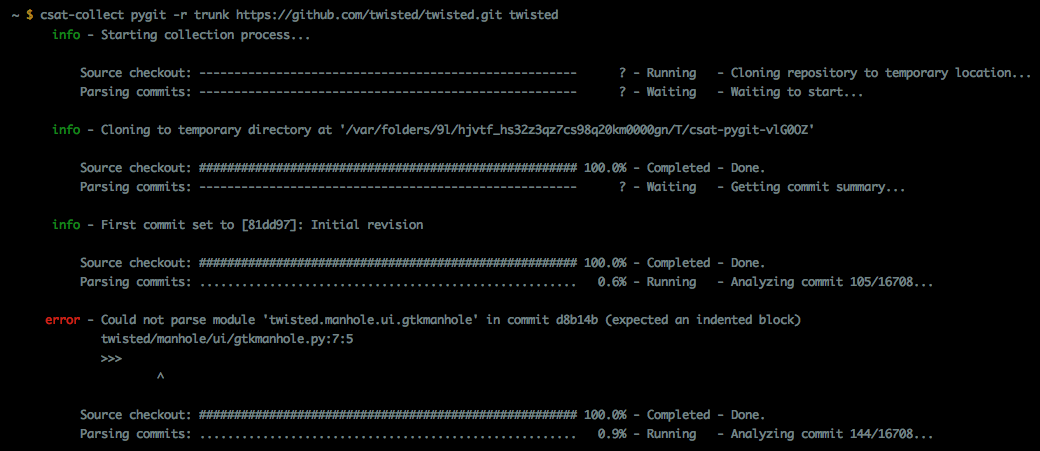
\includegraphics[width=\linewidth]{images/pygit-output}
  \caption[Example output of the \texttt{pygit} collector.]{Possible progress information of the \texttt{pygit} collector when run through the \texttt{csat-collect} command line utility.}
  \label{fig:pygit-output}
\end{figure}

\p{Acquisition server and \texttt{csat-collect}}
The second way to trigger the data acquisition process is to use the web application to configure an acquisition session and subsequently run it through the acquisition server. Normally, collector plugins, would then leverage the \texttt{csat-collect} utility to fulfill their job. This is the conventional way to collect data and the main use case around which the acquisition framework was designed.

\p{Acquisition server and other executables}
While the easiest way is to leverage the collector infrastructure provided by the framework, highly customized data collectors module can use their own executable to execute the data collection process. In fact, the usage of the \texttt{csat-collect} utility is completely opaque to the acquisition server, any executable found in the path can be used. In order to comply with the acquisition server collector interface, a third party executable has to follow this simple convention:

\begin{enumerate}
  \item It has to write a valid multi-domain GraphML document to its standard output file descriptor;
  \item It can make one-way \texttt{JSON-RPC} method calls by writing a correctly encoded \gls{json} payload to its standard error file descriptor;
  \item Any non-valid \gls{json} payload written to standard error is considered as informational output to be logged.
  \item It has to exit with a status code of $0$ if successful or $>0$ if an error arisen. In case of an error, no valid GraphML file has to be written.
\end{enumerate}

An example of this convention can easily be seen by executing any collector through \texttt{csat-\BreakableSlash{}collect} without connecting the standard error stream to a \gls{tty}. This can easily be emulated by piping all output to a second command as done in \vref{lst:pygit-out}.

\begin{userprompt}[basicstyle=\scriptsize\bf\ttfamily,caption={Example output of the \texttt{pygit} collector when run without a \gls{tty}},label=lst:pygit-out]
csat-collect pygit -r trunk https://github.com/twisted/twisted.git twisted 2>&1 | cat
\end{userprompt}
\begin{cmdresult}[basicstyle=\tiny\ttfamily]
2013-07-12 22:45:24,784 - INFO - runner - Starting collection process...
{"params": [0, {"status": 0, "statusText": "Waiting to start...", "progress": -1, "uuid": "bc9e035b-7b96-4e5f-858e-6e090eb88a33", "name": "Source checkout"}], "method": "updateTask"}
{"params": [1, {"status": 0, "statusText": "Waiting to start...", "progress": -1, "uuid": "bdfbb87c-3979-47e9-b061-e758624d3090", "name": "Parsing commits"}], "method": "updateTask"}
{"params": [0, {"status": 0, "statusText": "Cloning repository to temporary location...", "progress": -1, "uuid": "bc9e035b-7b96-4e5f-858e-6e090eb88a33", "name": "Source checkout"}], "method": "updateTask"}
{"params": [0, {"status": 1, "statusText": "Cloning repository to temporary location...", "progress": -1, "uuid": "bc9e035b-7b96-4e5f-858e-6e090eb88a33", "name": "Source checkout"}], "method": "updateTask"}
2013-07-12 22:45:24,788 - INFO - collector - Cloning to temporary directory at '/var/folders/9l/hjvtf_hs32z3qz7cs98q20km0000gn/T/csat-pygit-1gWVqn'
{"params": [0, {"status": 3, "statusText": "Done.", "progress": 1, "uuid": "bc9e035b-7b96-4e5f-858e-6e090eb88a33", "name": "Source checkout"}], "method": "updateTask"}
{"params": [1, {"status": 0, "statusText": "Getting commit summary...", "progress": -1, "uuid": "bdfbb87c-3979-47e9-b061-e758624d3090", "name": "Parsing commits"}], "method": "updateTask"}
2013-07-12 22:45:39,473 - INFO - collector - First commit set to [81dd97]: Initial revision
{"params": [1, {"status": 1, "statusText": "Getting commit summary...", "progress": 5.984798611526722e-05, "uuid": "bdfbb87c-3979-47e9-b061-e758624d3090", "name": "Parsing commits"}], "method": "updateTask"}
[...]
2013-07-12 22:45:42,745 - ERROR - collector - /Users/garetjax/Dropbox/CSAT/workspace/sources/csat/csat/collectors/pygit/collector.py:366 - Could not parse module 'twisted.manhole.ui.gtkmanhole' in commit d8b14b (expected an indented block)
2013-07-12 22:45:42,745 - ERROR - collector - /Users/garetjax/Dropbox/CSAT/workspace/sources/csat/csat/collectors/pygit/collector.py:366 - twisted/manhole/ui/gtkmanhole.py:7:5
2013-07-12 22:45:42,745 - ERROR - collector - /Users/garetjax/Dropbox/CSAT/workspace/sources/csat/csat/collectors/pygit/collector.py:366 - >>>
2013-07-12 22:45:42,745 - ERROR - collector - /Users/garetjax/Dropbox/CSAT/workspace/sources/csat/csat/collectors/pygit/collector.py:366 -         ^
{"params": [1, {"status": 1, "statusText": "Analyzing commit 106/16708...", "progress": 0.006284038542103058, "uuid": "bdfbb87c-3979-47e9-b061-e758624d3090", "name": "Parsing commits"}], "method": "updateTask"}
\end{cmdresult}


\subsection{Command line utilities}

\p{Introduction}
In the previous subsection we introduced the \texttt{csat-collect} command line utility. As seen, this utility allows to run any custom collector module currently hooked up to the framework. In addition to this command line utility, other utilities are provided as part of the framework, to either operate on acquired data or manage the web application.

\begin{description}
  \item[\texttt{csat-merge}] 
    \p{Other utilities}This command line utility takes two or more multi-domain graph files, merges them together and writes the result either to the standard output or to a specified file.
  \item[\texttt{csat-acquisition-server}] This utility allows to start or stop the acquisition server. Arguments can be used to set the public and private endpoints (\gls{tcp}, \gls{ssl}, interfaces, ports, \ldots) and to daemonize the server.
  \item[\texttt{csat-webserver}] This utility is the corresponding of the \texttt{csat-acquisition-server} for the web application server. It accepts a similar set of arguments.
  \item[\texttt{csat-init}] This command can be used to initialize a new \gls{csat} installation. It creates the environment and initializes the databases.
\end{description}

Additional information about all these utilities and their specific arguments can be found in the \emph{CSAT -- Usage and Administration Manual} document.

\subsection{Collector modules}

\p{Introduction}
In the present chapter we presented the analysis, design and implementation of the whole data acquisition framework. The role of the framework is to enable end users to easily collect data about their preferred systems, but one important piece is still missing: the data collection modules themselves. As part of the development of the framework, we also implemented six different data collection modules. In this last subsection we present foru of them and some of their peculiarities.

\subsubsection{The \texttt{pygit} collector}

\p{Overall graph structure}
The first collector we discuss is the \texttt{pygit} collector. We already used this module as use case for different examples throughout the chapter, notably in the class diagram represented in \vref{fig:class-collector}. This document analyzes the Python source code in a GIT repository \cite{git} and outputs a multi-domain graph with a domain for \emph{people} and one for \emph{components}. The different nodes are linked by two types of edges: a \emph{dependency} link between dependent components and \emph{modification} link between a person and any component it modified. No links are generated between people.

\p{Input parameters}
This collector requires two main arguments, namely the \gls{url} where the repository can be cloned from and the path to the Python source code relative to the repository root. Two optional parameters allow to fine tune the output. The first one allows to define a revision specifier (e.g., a specific branch to analyze, or an interval of commits), while the second is a binary switch to enable or disable the output of temporal data.

\p{Components and dependencies}
A node of type \emph{component} is created for each package and for each module in the Python source code tree. Each source code file is then parsed and its \texttt{import} statements extracted. If the import statement refers to another module in the project hierarchy, then a \emph{dependency} link is created between the current module and the imported module. Additional data, such as the developer which first introduced the dependency, and the date and commit in which it was added is registered as well.

\p{Developers and modifications}
While iterating over the commits in the given \texttt{revspec}, the collector also keeps track of all developers which contributed to the source code. Each time a new developer is encountered, a new \emph{person} node is added. For each commit, a link is made between the committer and the module it modified. The total number of commits is saved as an attribute of the node, while the number of times a module was modified by a given developer is saved as an attribute of the edge linking the two nodes.

\subsubsection{The \texttt{pipermail} collector}

\p{Overall graph structure}
The \texttt{pipermail} collector focuses on the analysis of mailing lists archives. It is named this way because it was built to parse archives generated by Pipermail, the mailing list archiver of the \emph{GNU Mailman} project \cite{mailman}. This collectors outputs a graph with a single domain for people, linked together if they interacted on the given mailing list.

\p{Input parameters}
The configuration of this module is very straightforward: the \gls{url} of the mailing lists archives is sufficient to complete the acquisition process. Optionally it is also possible to specify the degree of concurrency at which the archives are fetched from the remote server, but the default value already yields good results (the complete data collection process for the archives of a mailing list with \numprint{30000} messages can take less than 10 seconds; or less than 4 minutes for \numprint{650000} messages).

\p{People and interactions}
The collector creates a \emph{person} node for each person that ever wrote an email to the mailing list. A directed link is added between the author of each answer and the person which originally started the thread containing it. Additional stored data includes the total number of sent emails (on the nodes) and the number of unique threads in which an answer was provided (on the edges).

\subsubsection{The \texttt{ghcomments} collector}

\p{Data querying mechanism}
This third collectors analyzes a project residing on Github \cite{gh}. It works in a slightly different way than the previous two in that that instead of downloading readily available data, we make \gls{api} calls to a remote system \cite{ghapi} to query for the data we are interested into.

\p{Supported graph structures}
Another change in comparison with the previous collectors, is that this collector can output two different graphs, depending on how it is configured. In the first case, a multi-domain graph with two domains is created. One domains contains \emph{issues} (or \emph{change requests}) and the second contains people. A link is added between each issue and each person which \emph{created}, was assigned to (the \emph{assignee}), or \emph{closed} the issue itself. Additional links are added between an issue and each person that \emph{commented} on it. In the second case, a single-domain graph is created. The domain contains people, and links are created in a similar way to the \texttt{pipermail} collector: between each person which created the issue and any person which \emph{replied} to it.

\p{Input parameters}
This collector takes two main arguments: the Github path of the repository (normally in the form \texttt{<user>/<repo>}) and the desired output format. Two additional important options allow to specify an \gls{api} access token or the OAuth application \gls{id}. These are normally needed because Github limits \gls{api} calls to 60/hour for unauthenticated clients, while the limit for authenticated clients is raised to 5000/hour. It is also possible to specify this parameter as part of the web application configuration. The administration manual contains additional information about this topic.

\subsubsection{The \texttt{fileupload} collector}

\p{Collector goal}
The last collector we expound here presents an important difference with regard to the other three. In fact it only exposes the configuration interface but no data collection module. This behavior is due to its special nature. As easily guessable from its name, this collector allows the end user to upload an already available multi-domain GraphML document and can only be used from the web interface.

\p{Design}
To achieve this goal, we can exploit the object oriented design of the acquisition framework to provide a custom implementation of the \texttt{run} method of the \texttt{ICollectorConfigutator} interface, instead of using the default one provided by \texttt{ConfiguratorBase}. We can then present the interface already implemented for the \emph{Upload collector results} use case to the end user without really starting the data collection process.

\p{Implementation}
The implementation ends up being very simple. \Vref{lst:run-base} shows the default implementation as provided by the framework as default version for module specific \texttt{ICollector\BreakableSlash{}Configutator} realizations. \Vref{lst:run-upload} shows the overridden version as implemented by the \texttt{fileupload} collector.

\begin{lstlisting}[caption={Default implementation of the \texttt{run} method as found in the \texttt{ConfiguratorBase} class.},label=lst:run-base]
@implementer(ICollectorConfigurator, IPlugin)
class ConfiguratorBase(object):
    def run(self, request, model, remote):
        postback = model.create_postback_url(save=False)
        postback = request.build_absolute_uri(postback)
        command = self.get_command(model)
        model.running_instance_id = remote.runCollector(command, postback)
        model.set_running()
\end{lstlisting}

\begin{lstlisting}[caption={Custom implementation of the \texttt{run} method as found in the \texttt{UploadCollector} class.},label=lst:run-upload]
class UploadCollector(base.ConfiguratorBase):
    def run(self, request, model, remote):
        model.create_postback_url(save=True)
\end{lstlisting}


